\documentclass[12pt]{article}
\usepackage[T1]{fontenc}
\usepackage[utf8]{inputenc}
% Con una instalación completa de TeX se usa spanish.ldf; si falta, se usa el archivo .ini de babel.
\IfFileExists{spanish.ldf}{%
  \usepackage[spanish,es-tabla,es-nodecimaldot,es-noshorthands]{babel}%
}{%
  \usepackage[spanish,provide=*]{babel}%
  \setlocalecaption{spanish}{table}{Tabla}%
  \setlocalecaption{spanish}{listtable}{Índice de tablas}%
}
\usepackage{lmodern}
\usepackage{microtype}
\usepackage{amsmath, amssymb, amsthm}
\usepackage{bm}
\usepackage{graphicx}
\usepackage{float}
\usepackage{booktabs}
\usepackage{tabularx}
\usepackage{multirow}
\usepackage{array}
\usepackage{enumitem}
\usepackage{xcolor}
\usepackage{tikz}
\usetikzlibrary{arrows.meta,positioning,calc}
\usepackage{pgfplots}
\pgfplotsset{compat=1.18}
\usepackage[round,authoryear]{natbib}
\usepackage{xurl}
\usepackage[colorlinks=true,linkcolor=blue!50!black,citecolor=blue!50!black,urlcolor=blue!50!black]{hyperref}

\setlist{itemsep=2pt,topsep=4pt}
\setlength{\emergencystretch}{3em}
\newcolumntype{Y}{>{\raggedright\arraybackslash}X}
\newcolumntype{P}[1]{>{\raggedright\arraybackslash}p{#1}}

\theoremstyle{definition}
\newtheorem{hipotesis}{Hipótesis}
\newtheorem{invariante}{Invariante}

% Notación del modelo
\newcommand{\Pre}{\operatorname{Pre}}
\newcommand{\Rh}{\hat R}
\newcommand{\Sh}{\hat S}
\newcommand{\Lh}{\hat L}
\newcommand{\Pih}{\hat\Pi}
\newcommand{\rstar}{r^{\ast}}
\newcommand{\Slisto}{S_{\mathrm{listo}}}
\newcommand{\Smin}{S_{\min}}
\newcommand{\Hist}{\mathcal H}
\newcommand{\Dom}{\mathcal D}
\newcommand{\Banco}{\mathcal B}
\newcommand{\Carga}{\mathcal L}

\definecolor{azul}{HTML}{2A78D6}
\definecolor{naranja}{HTML}{EB6834}
\definecolor{verde}{HTML}{1B8F66}
\definecolor{gris}{HTML}{52514E}
\definecolor{morado}{HTML}{6250D6}

\begin{document}

%=====================================================================
% Portada
%=====================================================================
\begin{titlepage}
\begin{center}

\IfFileExists{logouaemex.png}{
\includegraphics[width=3.2cm]{logouaemex}\par}{%
\IfFileExists{logouaemex.jpg}{
\includegraphics[width=3.2cm]{logouaemex}\par}{%
\IfFileExists{logouaemex.pdf}{
\includegraphics[width=3.2cm]{logouaemex}\par}{}}}

\vspace{0.2cm}
{\large \textbf{MAESTRÍA EN INTELIGENCIA ARTIFICIAL APLICADA}}

\vspace{1.5cm}
{\large \textbf{PROTOCOLO DE INVESTIGACIÓN}}

\vspace{1.5cm}
{\large \textbf{Plataforma web inteligente de repetición espaciada con algoritmo adaptativo para mejorar la retención de habilidades procedimentales en física de bachillerato}}

\vspace{2.5cm}
\setlength{\tabcolsep}{0.5cm}
\renewcommand{\arraystretch}{1.2}
\begin{tabular}{r l}
\textbf{Nombre del alumno:} & Act. Gustavo Sánchez de la Rosa \\[0.5cm]
\textbf{Director de tesis:} & Dr. Marco Antonio Ramos Corchado \\[0.5cm]
\textbf{Codirectora:} & Dra. Vianney Muñoz Jiménez \\[0.5cm]
\textbf{Tutor:} & Dr. Héctor Caballero Hernández
\end{tabular}

\vspace{2cm}
{\small Fecha de inicio: febrero de 2026}\\
{\small Última actualización: noviembre de 2026}

\vfill
\end{center}
\end{titlepage}

%=====================================================================
\section*{Resumen}
%=====================================================================

Los sistemas de repetición espaciada se diseñaron para memorizar hechos aislados: cada tarjeta ejercita una sola pieza de conocimiento y es independiente de las demás. Resolver un problema de física es distinto, porque exige ejecutar varios procedimientos que dependen unos de otros. Este proyecto propone un modelo y una plataforma web para planificar la práctica de \emph{habilidades procedimentales}, con la mecánica clásica de bachillerato como primer dominio. El modelo combina cuatro piezas: un grafo de prerrequisitos con una matriz $Q$ fraccional, el modelo de olvido exponencial con la dinámica de saltos de \citet{tabibian2019}, un modelo de observación conjuntivo con descuido y adivinanza que permite repartir la culpa de un fallo entre las habilidades de un problema, y un planificador diario que admite temas nuevos solo cuando sus prerrequisitos están consolidados y la carga de repaso cabe en el tiempo disponible. Los parámetros se estiman por máxima verosimilitud.

A la fecha de esta actualización el modelo está formulado, se evaluó con un simulador Monte Carlo y existe un prototipo funcional. En simulación, sobre un grafo de 168 subtemas de mecánica, el sistema supera a una política tipo Anki SM-2 en la probabilidad media de resolver un problema nuevo 30 días después del curso ($+0.090$ y $+0.047$ según el escenario), sobre todo porque introduce más temas. La ventaja desaparece si el grafo contiene dependencias falsas y no aparece cuando el temario se describe con pocas unidades gruesas. La segunda mitad de la tesis valida el grafo con docentes, calibra el modelo con un piloto real y compara el sistema contra una política de referencia en un experimento intrasujeto con estudiantes de bachillerato.

\vspace{0.5cm}
\noindent\textbf{Palabras clave:} repetición espaciada, habilidades procedimentales, grafo de prerrequisitos, modelos de estudiante, optimización submodular, física de bachillerato.

\newpage
\tableofcontents
\newpage

%=====================================================================
\section{Introducción}
%=====================================================================

El examen de admisión a la universidad es, para muchos estudiantes de bachillerato, un filtro que define sus opciones académicas. Una parte importante de esos exámenes no pide recordar un dato, sino resolver un problema: plantear la situación, elegir un procedimiento, ejecutarlo paso a paso y verificar el resultado. Esas habilidades no se adquieren releyendo apuntes ni estudiando la noche anterior; se adquieren con práctica distribuida en el tiempo.

La repetición espaciada es una de las estrategias de aprendizaje con mejor respaldo experimental. Distribuir la práctica en el tiempo mejora la retención a largo plazo frente al estudio concentrado \citep{cepeda2006,kang2016}, y el beneficio aumenta cuando cada repaso exige recuperar activamente lo aprendido. Los sistemas computacionales de repetición espaciada, de SM-2 \citep{wozniak1990} a FSRS \citep{ye2022}, y los enfoques de control óptimo como MEMORIZE \citep{tabibian2019} deciden \emph{cuándo} repasar cada elemento para que no se olvide.

Todos esos sistemas comparten un supuesto: cada elemento que se repasa es independiente y ejercita una sola pieza de conocimiento. \citet{choffin2021} señalan que, hasta donde saben, todos los algoritmos de espaciado adaptativo están pensados para elementos de un solo componente. Resolver un problema de física rompe ese supuesto de tres maneras:

\begin{enumerate}[label=(\alph*)]
\item un problema de tiro parabólico exige recuperar a la vez la descomposición de vectores, las ecuaciones del movimiento acelerado y la independencia de los movimientos horizontal y vertical, así que cada intento aporta evidencia sobre varias habilidades;
\item un fallo no indica cuál de esas habilidades falló;
\item existe un orden natural de aprendizaje: introducir un tema antes de que sus bases estén firmes desperdicia práctica, e introducir demasiados temas a la vez satura la cola de repasos \citep{reddy2016}.
\end{enumerate}

Esta tesis propone un sistema que conserva la idea central de la repetición espaciada (repasar justo cuando el recuerdo empieza a debilitarse) y la extiende a \emph{habilidades repetibles}: procedimientos que se ejecutan una y otra vez sobre datos distintos. El sistema se apoya en un grafo de prerrequisitos del temario, en un modelo de memoria por habilidad y en un planificador que decide cada día qué repasar y qué tema nuevo introducir.

\paragraph{Cambios respecto a la versión anterior del protocolo.} La primera versión de este protocolo (junio de 2026) planteaba una plataforma para cuatro disciplinas (matemáticas, física, química y biología) y proponía adaptar la regresión de vida media \citep{settles2016} con predictores como el tiempo de resolución o el tipo de error. Durante el primer año el proyecto avanzó en otra dirección, más acotada y más precisa:

\begin{itemize}
\item el alcance se redujo a la \textbf{física clásica (mecánica) de bachillerato}, organizada como un grafo de 15 unidades y 168 subtemas (sección~\ref{sec:dominio});
\item se formuló un \textbf{modelo propio} que integra el grafo de prerrequisitos con el modelo de memoria de \citet{tabibian2019} (sección~\ref{sec:modelo});
\item el modelo se \textbf{evaluó por simulación} y se construyó un \textbf{prototipo funcional} (sección~\ref{sec:avances});
\item la validación se rediseñó como un \textbf{piloto de calibración} seguido de un \textbf{experimento intrasujeto} (sección~\ref{sec:metodologia}).
\end{itemize}

El resto del documento se organiza así. La sección~\ref{sec:marco} presenta el marco teórico y la~\ref{sec:estado} el estado del arte. Las secciones~\ref{sec:problema} a~\ref{sec:justificacion} plantean el problema, las preguntas de investigación, la meta de ingeniería, los objetivos y la justificación. La sección~\ref{sec:propuesta} describe la propuesta de solución y la~\ref{sec:avances} los avances. Las secciones~\ref{sec:metodologia} y~\ref{sec:cronograma} presentan la metodología y el cronograma.

%=====================================================================
\section{Marco teórico}
\label{sec:marco}
%=====================================================================

Esta sección reúne las bases cognitivas y computacionales del proyecto. Se organiza en cuatro bloques: los fenómenos de la memoria que la repetición espaciada aprovecha, los algoritmos que la implementan, los modelos de estudiante que describen problemas con varias habilidades y la herramienta de optimización que usa el planificador.

\subsection{Memoria, espaciamiento y práctica}

\subsubsection{Repetición espaciada}

La \textbf{repetición espaciada} reparte en el tiempo las sesiones dedicadas a un mismo contenido, con intervalos que crecen a medida que el recuerdo se consolida. Se apoya en el \textbf{efecto de espaciamiento}, descrito por Ebbinghaus en 1885: con el mismo tiempo total de estudio, la retención a largo plazo es mayor cuando la práctica se distribuye que cuando se concentra en una sola sesión \citep{kang2016}. Un metaanálisis de cientos de experimentos confirma el efecto y muestra que el intervalo óptimo entre repasos crece con el plazo en el que se quiere recordar \citep{cepeda2006,cepeda2008}. En los sistemas digitales, un algoritmo decide cuándo presentar de nuevo cada elemento a partir del historial de desempeño del usuario.

\subsubsection{Curva del olvido y modelos de memoria}

La \textbf{curva del olvido} describe cómo baja la probabilidad de recordar algo con el tiempo transcurrido desde el último repaso. La forma más usada en los algoritmos es la exponencial,
\[
m(t)=e^{-n\,\Delta t},
\]
donde $\Delta t$ es el tiempo desde el último repaso y $n>0$ es la \textbf{tasa de olvido} \citep{settles2016,tabibian2019}. Su inversa, $S=1/n$, se llama \textbf{estabilidad} y se mide en días: es el tiempo en el que el recuerdo cae a $e^{-1}\approx0.37$. La \textbf{vida media}, el tiempo en que cae a $0.5$, vale $S\ln2$.

La forma exponencial supone que la tasa de olvido es constante entre repasos. Los datos de memoria humana se ajustan a menudo mejor a una \textbf{ley de potencia}, que decae más despacio en la cola. Este proyecto usa la forma exponencial en el modelo, porque permite derivaciones cerradas, y la ley de potencia en el simulador, para medir el costo de ese supuesto (sección~\ref{sec:avances}).

\subsubsection{Efecto de retraso y esfuerzo de recuperación}

El \textbf{efecto de retraso} (\emph{lag effect}) precisa que, con el mismo número de repeticiones, intervalos más largos (hasta cierto límite) producen mejor retención \citep{cepeda2008}. La \textbf{hipótesis del esfuerzo de recuperación} ofrece una explicación: recuperar con éxito algo que ya empezaba a olvidarse fortalece la memoria más que recuperar algo fresco \citep{pyc2009}. Esta hipótesis es la base de la regla de actualización tras un acierto del modelo propuesto (ecuación~\ref{eq:acierto}).

\subsubsection{Práctica de recuperación}

La \textbf{práctica de recuperación} (\emph{testing effect}) es el hallazgo de que evocar activamente un contenido produce mejor retención que releerlo \citep{kang2016}. En el dominio procedimental, recuperar significa resolver un problema sin consultar la solución. Por eso la plataforma presenta problemas abiertos con respuesta numérica, y no tarjetas con la respuesta en el reverso.

\subsubsection{Conocimiento declarativo y procedimental}

La psicología cognitiva distingue el \textbf{conocimiento declarativo} (saber qué: hechos, conceptos, definiciones) del \textbf{conocimiento procedimental} (saber cómo: resolver una ecuación, aplicar la segunda ley de Newton). El segundo se adquiere con práctica repetida y retroalimentación, y su decaimiento con el desuso está documentado \citep{arthur1998}, aunque la forma funcional de ese decaimiento no está establecida. La evidencia de que el espaciamiento mejora el aprendizaje de procedimientos existe, sobre todo en matemáticas \citep{rohrer2007,rohrer2015}, pero es menos robusta que para hechos \citep{barzagar2019}.

\subsubsection{Resolución de problemas y práctica intercalada}

Un problema de física exige representar la situación, seleccionar los principios aplicables, ejecutar los procedimientos y verificar el resultado. La \textbf{práctica bloqueada} resuelve muchos problemas del mismo tipo seguidos; la \textbf{práctica intercalada} alterna tipos distintos en una misma sesión. La intercalada produce peor desempeño durante la práctica, pero mejor retención y, sobre todo, mejor capacidad para reconocer qué procedimiento aplicar \citep{rohrer2007,rohrer2015}. Un sistema que repasa varias habilidades por sesión intercala de forma natural.

\subsubsection{Teoría de la carga cognitiva}

La \textbf{teoría de la carga cognitiva} sostiene que la memoria de trabajo tiene una capacidad limitada y que el aprendizaje se dificulta cuando la demanda de la tarea la excede \citep{sweller1988}. Automatizar los procedimientos elementales (despejar, descomponer un vector, convertir unidades) libera memoria de trabajo para los aspectos nuevos de un problema. Esta es una razón cognitiva para no introducir un tema antes de que sus prerrequisitos estén consolidados, que el modelo implementa con la regla de admisión (ecuación~\ref{eq:admision}).

\subsection{Algoritmos de repetición espaciada}

\subsubsection{Sistema Leitner}

El \textbf{sistema Leitner}, propuesto por Sebastian Leitner en la década de 1970, organiza las tarjetas en cajas que se repasan con periodicidad fija y creciente. Un acierto sube la tarjeta a la caja siguiente; un error la regresa a la primera. Es fácil de implementar, pero no se ajusta al ritmo de olvido de cada persona ni de cada tarjeta.

\subsubsection{SM-2}

El algoritmo \textbf{SM-2} \citep{wozniak1990}, creado por Piotr Woźniak para el programa SuperMemo, calcula el siguiente intervalo multiplicando el anterior por un \emph{factor de facilidad} propio de cada tarjeta, que se ajusta según la calificación que el usuario da a su recuerdo (de 0 a 5). Los intervalos iniciales son de 1 y 6 días. Sus sucesores en SuperMemo incorporan modelos explícitos de estabilidad y recuperabilidad.

\subsubsection{Anki y FSRS}

\textbf{Anki} es un programa de código abierto de tarjetas de estudio. Durante años su planificador fue una variante de SM-2 con cuatro botones de autoevaluación («De nuevo», «Difícil», «Bien», «Fácil»). Desde 2023 incluye además \textbf{FSRS} (\emph{Free Spaced Repetition Scheduler}), un modelo de tres variables por tarjeta (dificultad, estabilidad y recuperabilidad) cuyos parámetros se ajustan con el historial del usuario \citep{ye2022,su2023}. Anki es muy usado en medicina y en idiomas \citep{gilbert2023,jape2022,hanson2020}, dominios mayormente declarativos.

\subsubsection{Regresión de vida media (HLR)}

La \textbf{regresión de vida media} de \citet{settles2016} estima la vida media de una palabra en la memoria del estudiante como $h=2^{\bm\Theta\cdot\mathbf x}$, donde $\mathbf x$ resume el historial (aciertos y errores previos) y rasgos del elemento, y predice el recuerdo como $p=2^{-\Delta t/h}$. Los pesos $\bm\Theta$ se ajustan con datos. Con datos de Duolingo, HLR redujo más de 45\,\% el error de predicción frente a Leitner y Pimsleur, y en un estudio operativo aumentó 12\,\% la participación diaria de los estudiantes.

\subsubsection{Control óptimo estocástico: MEMORIZE}

\citet{tabibian2019} plantean la programación de repasos como un problema de control óptimo estocástico. Los repasos son un proceso puntual con intensidad $u(t)$, y el recuerdo sigue una ecuación diferencial estocástica con saltos: decae exponencialmente entre repasos y, en cada repaso, salta de vuelta a 1,
\[
dm(t)=-n(t)\,m(t)\,dt+\bigl(1-m(t)\bigr)\,dN(t).
\]
Tras cada repaso, la tasa de olvido se multiplica por $(1-\alpha)$ si se acierta y por $(1+\beta)$ si se falla. Con una pérdida cuadrática, la intensidad óptima resulta proporcional a la probabilidad de haber olvidado: $u^\ast(t)\propto1-m(t)$. El algoritmo resultante se llama \textbf{MEMORIZE}. Con datos de Duolingo, los estudiantes cuyos repasos se parecían más al calendario de MEMORIZE olvidaban menos. \citet{upadhyay2021} lo validaron después con un experimento aleatorizado a gran escala.

\subsubsection{Red de colas de Leitner}

\citet{reddy2016} modelan el sistema Leitner como una red de colas en la que las tarjetas pasan de una caja a otra según las respuestas. El modelo predice una \textbf{transición de fase}: existe una tasa máxima de introducción de material nuevo; por debajo de ella el sistema es estable, y por encima los elementos se acumulan en las primeras cajas y el aprendizaje neto se desploma. Este resultado motiva el control de carga del modelo propuesto (ecuación~\ref{eq:carga}).

\subsection{Modelos de estudiante y estructura del conocimiento}

\subsubsection{Teoría de respuesta al ítem}

La \textbf{teoría de respuesta al ítem} (TRI) agrupa modelos psicométricos que relacionan la probabilidad de responder bien con rasgos del ítem (dificultad, discriminación, probabilidad de acertar por azar) y con la habilidad latente de la persona. Sus modelos son estáticos: describen el desempeño en un momento, no cómo cambia con la práctica y el olvido. En este proyecto la TRI aporta la idea de que la dificultad de un ítem y la habilidad del estudiante pueden estimarse a partir de los datos; su extensión natural es el modelo jerárquico de la sección~\ref{sec:estimacion}.

\subsubsection{Rastreo bayesiano del conocimiento: descuido y adivinanza}

El \textbf{rastreo bayesiano del conocimiento} (BKT) de \citet{corbett1994} modela si un estudiante domina una habilidad como un estado oculto que se actualiza con cada respuesta. Introduce dos parámetros de observación que el modelo propuesto adopta: el \textbf{descuido} $s$ (\emph{slip}), la probabilidad de fallar aunque se domine la habilidad, y la \textbf{adivinanza} $g$ (\emph{guess}), la probabilidad de acertar sin dominarla.

\subsubsection{Matriz $Q$ y modelos conjuntivos}

La \textbf{matriz $Q$} \citep{tatsuoka1983} indica qué habilidades requiere cada ítem: $q_{jk}=1$ si el ítem $j$ requiere la habilidad $k$. Los \textbf{modelos conjuntivos} de diagnóstico cognitivo, como DINA \citep{junker2001} y su generalización G-DINA \citep{delatorre2011}, suponen que responder bien exige dominar \emph{todas} las habilidades requeridas, con descuido y adivinanza como ruido. Las alternativas aditivas, como AFM \citep{cen2006} y PFA \citep{pavlik2009}, suman las contribuciones de cada habilidad. El marco KLI \citep{koedinger2012} llama \emph{componentes de conocimiento} a estas unidades y advierte que su granularidad es una cuestión empírica, lo cual resultó decisivo en este proyecto (sección~\ref{sec:avances}).

\subsubsection{Espacios de conocimiento}

La \textbf{teoría de espacios de conocimiento} \citep{doignon1985} describe el conocimiento de un estudiante como el conjunto de ítems que domina, restringido por relaciones de prerrequisito. El \textbf{borde externo} (\emph{outer fringe}) de ese conjunto son los ítems que el estudiante está listo para aprender: aquellos cuyos prerrequisitos ya domina. La regla de admisión del modelo propuesto es un borde externo en el que «domina» se sustituye por «tiene una memoria suficientemente estable».

\subsection{Optimización submodular}

Una función de conjuntos $V$ es \textbf{submodular} si agregar un elemento a un conjunto pequeño aporta al menos tanto como agregarlo a uno más grande que lo contiene (rendimientos decrecientes). Si además es monótona y no negativa, el algoritmo voraz que agrega en cada paso el elemento de mayor ganancia marginal alcanza al menos una fracción $1-1/e\approx0.63$ del óptimo bajo una restricción de cardinalidad \citep{nemhauser1978}. \citet{hunziker2019} usan esta propiedad para enseñar varios conceptos a un aprendiz que olvida. El planificador propuesto la usa para elegir los problemas de cada sesión (ecuación~\ref{eq:cobertura}).

%=====================================================================
\section{Estado del arte}
\label{sec:estado}
%=====================================================================

\subsection{Evidencia empírica del espaciamiento}

La base empírica de la repetición espaciada es amplia. \citet{cepeda2006} sintetizan cientos de experimentos de recuerdo verbal y confirman el efecto de espaciamiento; \citet{cepeda2008} muestran que el intervalo óptimo depende del plazo de retención. \citet{kang2016} resume la evidencia para el diseño de políticas educativas y señala que el espaciado beneficia no solo la memoria, sino también la resolución de problemas y la transferencia, y que combinarlo con práctica de recuperación amplifica el efecto.

En matemáticas, intercalar y espaciar problemas mejora el desempeño en pruebas diferidas \citep{rohrer2007,rohrer2015}. Sin embargo, al llevar el espaciamiento de la práctica matemática al aula con estudiantes de tercero y séptimo grado, \citet{barzagar2019} muestran que la evidencia en dominios procedimentales es menos consistente que para hechos.

En física, \citet{voice2020} incorporaron una aplicación web de repetición espaciada en un curso universitario de termodinámica. Los estudiantes que la usaron de forma espaciada obtuvieron 70\,\% en el examen final frente a 61\,\% de quienes no la usaron, y 45\,\% frente a 34\,\% en una evaluación aplicada después de las vacaciones. El estudio es observacional (los estudiantes eligieron cómo usar la herramienta) y su calendario de repasos era predefinido, no ajustado a cada estudiante.

\citet{yuan2022} revisa la evidencia del efecto de espaciamiento en la educación científica desde la neurociencia, la cognición y la metacognición, y explica por qué estudiantes y docentes siguen prefiriendo el estudio concentrado: la fluidez inmediata se confunde con aprendizaje duradero. \citet{mostrady2025} revisan el microaprendizaje (contenido en unidades muy pequeñas) y advierten que no es adecuado para temas que requieren integración profunda y que puede generar una falsa sensación de dominio. \citet{xu2023} revisan el aprendizaje basado en juegos en educación médica, que combina retroalimentación, evaluación y repetición espaciada con participación activa; la mayoría de los estudios que revisan miden satisfacción o conocimiento inmediato, no retención a largo plazo.

En educación médica, \citet{jape2022} desarrollaron un mazo de Anki para farmacología con un diseño mixto (encuesta, grupos focales e intervención) y reportaron buena aceptación por parte de los estudiantes. \citet{gilbert2023}, en un estudio de cohorte con estudiantes de medicina, encontraron una asociación entre el uso de Anki y mejores puntajes en exámenes estandarizados, sin asignación aleatoria. \citet{hanson2020} encontraron efectos positivos de Anki en el aprendizaje de español como segunda lengua, pero con baja adherencia voluntaria.

La evidencia de mayor escala proviene de \citet{price2025}: 26\,258 médicos familiares y residentes asignados aleatoriamente a un grupo sin repetición espaciada o a una de cinco condiciones con repetición. La repetición espaciada mejoró el aprendizaje (58.03\,\% frente a 43.20\,\%, $d=0.62$) y, en menor medida, la transferencia a casos clínicos nuevos (58.33\,\% frente a 52.39\,\%). El estudio usa preguntas de opción múltiple sobre contenido clínico, no resolución abierta de problemas.

\subsection{Modelos computacionales de planificación}

En paralelo se desarrollaron modelos para decidir cuándo repasar. HLR \citep{settles2016} hizo de la vida media de cada elemento una cantidad que se aprende de los datos. MEMORIZE \citep{tabibian2019} derivó la intensidad óptima de repaso, proporcional a la probabilidad de olvido, y \citet{upadhyay2021} adaptaron el enfoque para elegir qué elementos repasar dentro de sesiones elegidas por el usuario, con un experimento aleatorizado a gran escala. \citet{reddy2016} mostraron la transición de fase que aparece cuando se introduce material nuevo más rápido de lo que el sistema puede procesar. FSRS \citep{ye2022,su2023}, hoy integrado en Anki, modela dificultad, estabilidad y recuperabilidad y elige los intervalos resolviendo un problema de ruta más corta estocástica. \citet{hunziker2019} dan garantías de aproximación para enseñar varios conceptos a un aprendiz que olvida mediante funciones submodulares.

Todos estos modelos suponen elementos independientes de una sola pieza de conocimiento (palabras, tarjetas, preguntas). El propio trabajo de \citet{tabibian2019} deja como trabajo futuro el caso de elementos dependientes entre sí.

\subsection{Elementos con varias habilidades y estructura de prerrequisitos}

Un grupo más reducido de trabajos aborda elementos que ejercitan varias habilidades. DAS3H \citep{choffin2019} extiende los modelos aditivos de factores con ventanas temporales de olvido por habilidad, de modo que la predicción de un ítem combina el historial de todas las habilidades que involucra. \citet{choffin2021} extienden heurísticas de espaciado a ítems con varias habilidades mediante una selección voraz de subconjuntos; es el antecedente más cercano al planificador de este proyecto, aunque no incorpora prerrequisitos ni control de carga. La plataforma comercial Math Academy describe un esquema propietario, \emph{Fractional Implicit Repetition}, en el que el crédito por resolver un tema avanzado «fluye» fraccionalmente hacia los temas que usa \citep{skycak2023}. Hasta donde sabemos, ese esquema no tiene un modelo publicado ni una evaluación controlada.

\subsection{Limitaciones de la investigación actual y oportunidades}

De la revisión se desprenden cuatro vacíos que justifican esta investigación:

\begin{enumerate}
\item \textbf{Elementos independientes.} Los algoritmos de repetición espaciada con fundamento formal (HLR, MEMORIZE, FSRS, la red de colas de Leitner) suponen elementos de un solo componente \citep{settles2016,tabibian2019,ye2022,reddy2016}. No modelan que un problema ejercite varias habilidades, ni reparten la evidencia de un fallo entre ellas.

\item \textbf{Prerrequisitos y saturación.} Los trabajos con varias habilidades \citep{choffin2019,choffin2021} no usan la estructura de prerrequisitos para decidir cuándo introducir un tema, y los modelos de estructura del conocimiento \citep{doignon1985} no modelan el olvido. El único esquema que combina ambas cosas \citep{skycak2023} es propietario y no está evaluado.

\item \textbf{Población y dominio.} Los estudios empíricos se concentran en estudiantes universitarios de medicina \citep{gilbert2023,jape2022}, física \citep{voice2020} o idiomas \citep{hanson2020}, y en profesionales \citep{price2025}. Hay poca evidencia con estudiantes de bachillerato y con resolución abierta de problemas de física.

\item \textbf{Validación.} Los estudios con herramientas existentes son observacionales o comparan contra no practicar. Falta comparar, con tiempo de práctica igualado, una política diseñada para habilidades procedimentales contra una política de repetición espaciada estándar.
\end{enumerate}

Las Tablas~\ref{tab:modelos} a~\ref{tab:multi} resumen los trabajos revisados.

\begin{table}[H]
\centering\small
\caption{Modelos computacionales y algoritmos de repetición espaciada.}
\label{tab:modelos}
\begin{tabularx}{\textwidth}{@{}P{2.7cm}YYY@{}}
\toprule
\textbf{Autores (año)} & \textbf{Aporte} & \textbf{Tipo de conocimiento} & \textbf{Limitación} \\
\midrule
\citet{settles2016} & HLR: vida media entrenable a partir del historial & Factual (vocabulario) & Elementos independientes; solo idiomas \\
\citet{tabibian2019} & MEMORIZE: control óptimo, $u^\ast\propto1-m$ & Factual (vocabulario) & Elementos independientes; sin prerrequisitos \\
\citet{reddy2016} & Red de colas de Leitner y transición de fase & Factual & Elementos independientes \\
\citet{ye2022}; \citet{su2023} & FSRS: dificultad, estabilidad y recuperabilidad & Factual (tarjetas) & Elementos independientes \\
\citet{upadhyay2021} & Selección de elementos dentro de sesiones; experimento aleatorizado & Factual & Elementos independientes \\
\bottomrule
\end{tabularx}
\end{table}

\begin{table}[H]
\centering\small
\caption{Revisiones y aplicaciones en dominios mayormente factuales.}
\label{tab:revisiones}
\begin{tabularx}{\textwidth}{@{}P{2.7cm}YYY@{}}
\toprule
\textbf{Autores (año)} & \textbf{Aporte} & \textbf{Tipo de conocimiento} & \textbf{Limitación} \\
\midrule
\citet{gilbert2023} & Cohorte: uso de Anki y exámenes en medicina & Factual & Sin aleatorización; universitarios \\
\citet{hanson2020} & Anki en español como segunda lengua & Factual (vocabulario) & Baja adherencia voluntaria \\
\citet{kang2016} & Revisión para políticas educativas & Revisión & Sin implementación propia \\
\citet{mostrady2025} & Revisión del microaprendizaje & Factual y procedimental simple & Poco adecuado para temas que requieren integración \\
\citet{xu2023} & Revisión de aprendizaje basado en juegos en medicina & Factual y procedimental & Poca medición de retención a largo plazo \\
\citet{yuan2022} & Espaciamiento en ciencia: mecanismos y barreras & Revisión & Sin implementación propia \\
\bottomrule
\end{tabularx}
\end{table}

\begin{table}[H]
\centering\small
\caption{Estudios aplicados a dominios procedimentales.}
\label{tab:procedimental}
\begin{tabularx}{\textwidth}{@{}P{2.7cm}YYY@{}}
\toprule
\textbf{Autores (año)} & \textbf{Aporte} & \textbf{Tipo de conocimiento} & \textbf{Limitación} \\
\midrule
\citet{voice2020} & Aplicación web de repetición espaciada en termodinámica & Procedimental (física universitaria) & Observacional; calendario fijo, no adaptativo \\
\citet{jape2022} & Mazo de Anki para farmacología & Factual y algo procedimental & Autoevaluación subjetiva \\
\citet{price2025} & Ensayo aleatorizado con 26\,258 médicos & Aplicación clínica & Opción múltiple; un solo dominio \\
\citet{rohrer2015} & Práctica intercalada en matemáticas, en el aula & Procedimental (secundaria) & Calendario fijo, no adaptativo \\
\citet{barzagar2019} & Espaciamiento de práctica matemática en el aula & Procedimental (primaria y secundaria) & Calendario fijo; efectos menos consistentes que con hechos \\
\bottomrule
\end{tabularx}
\end{table}

\begin{table}[H]
\centering\small
\caption{Modelos para elementos con varias habilidades o con estructura de prerrequisitos.}
\label{tab:multi}
\begin{tabularx}{\textwidth}{@{}P{2.7cm}YYY@{}}
\toprule
\textbf{Autores (año)} & \textbf{Aporte} & \textbf{Qué modela} & \textbf{Qué le falta para este problema} \\
\midrule
\citet{choffin2019} & DAS3H: predicción con olvido por habilidad & Varias habilidades por ítem & Planificación con prerrequisitos y carga \\
\citet{choffin2021} & Heurísticas de espaciado para ítems con varias habilidades & Varias habilidades; selección voraz & Prerrequisitos; control de carga \\
\citet{skycak2023} & Repetición implícita fraccional (Math Academy) & Crédito fraccional sobre un grafo & Modelo publicado; evaluación controlada \\
\citet{doignon1985} & Espacios de conocimiento; borde externo & Prerrequisitos & Olvido \\
\citet{junker2001}; \citet{delatorre2011} & DINA y G-DINA & Modelo conjuntivo con matriz $Q$ & Dinámica temporal \\
\bottomrule
\end{tabularx}
\end{table}

%=====================================================================
\section{Planteamiento del problema}
\label{sec:problema}
%=====================================================================

Los estudiantes de bachillerato que se preparan para un examen de admisión suelen estudiar física de dos maneras poco eficaces: concentran la práctica en las semanas previas al examen y resuelven muchos problemas del mismo tipo seguidos. Ambas producen una sensación de dominio que no dura y no desarrollan la capacidad de reconocer qué procedimiento aplicar cuando los problemas aparecen mezclados \citep{kang2016,yuan2022}.

La repetición espaciada ataca justamente esos dos defectos, pero las herramientas que la implementan fueron diseñadas para tarjetas independientes. Aplicadas a la física, enfrentan tres problemas técnicos que ninguna resuelve en conjunto:

\begin{enumerate}
\item \textbf{Crédito.} Un problema de caída libre ejercita por completo la caída libre y, de paso, las ecuaciones del movimiento acelerado. Una herramienta de tarjetas solo registra el repaso del tema principal y sigue programando repasos innecesarios de sus prerrequisitos.
\item \textbf{Culpa.} Si el estudiante falla, el error puede venir de cualquiera de las habilidades que el problema usa. Castigar a todas por igual, o solo al tema principal, distorsiona el calendario.
\item \textbf{Orden y saturación.} Un tema introducido sobre bases frágiles se aprende mal, y cada tema introducido agrega repasos futuros. Sin una regla que coordine ambas cosas, el sistema avanza demasiado rápido y se satura \citep{reddy2016}, o avanza demasiado lento y no cubre el temario.
\end{enumerate}

Los modelos computacionales disponibles resuelven partes aisladas: MEMORIZE y FSRS el momento del repaso, DAS3H la predicción con varias habilidades, la teoría de espacios de conocimiento el orden. No existe un modelo publicado y evaluado que integre la dinámica de la memoria, el crédito y la culpa entre habilidades, el orden de prerrequisitos y el control de carga, ni una plataforma que lo implemente para la física de bachillerato. Este trabajo aborda ese vacío con la mecánica clásica como primer dominio.

%=====================================================================
\section{Preguntas de investigación e hipótesis}
\label{sec:preguntas}
%=====================================================================

\subsection{Preguntas de investigación}

\begin{enumerate}[label=P\arabic*.]
\item ¿Cómo se puede extender un modelo de repetición espaciada con fundamento en control óptimo \citep{tabibian2019} a problemas que ejercitan varias habilidades relacionadas por prerrequisitos?
\item ¿Qué componentes del modelo (crédito a prerrequisitos, reparto de culpa, compuerta de prerrequisitos, control de carga) aportan al aprendizaje simulado, y bajo qué condiciones del dominio?
\item ¿Con qué precisión predice el modelo, calibrado con datos de un piloto, el desempeño de estudiantes reales de bachillerato?
\item Con el mismo tiempo de práctica, ¿los estudiantes retienen más habilidades de mecánica a 30 días con el sistema propuesto que con una política de repetición espaciada estándar?
\end{enumerate}

\subsection{Hipótesis}

\begin{hipotesis}[principal]
\label{h:principal}
En una prueba diferida a 30 días con problemas nuevos, la proporción de aciertos en los subtemas practicados con el sistema propuesto es mayor que en los practicados con la política de referencia (SM-2 o FSRS con límite de temas nuevos por día), con el mismo número de problemas por sesión.
\end{hipotesis}

\begin{hipotesis}[mecanismo]
\label{h:mecanismo}
La ventaja de la hipótesis~\ref{h:principal} se explica principalmente por una mayor cobertura (más subtemas introducidos durante el curso) y no por una mayor retención en cada subtema introducido.
\end{hipotesis}

\begin{hipotesis}[modelo]
\label{h:modelo}
Con los datos del piloto, el modelo con crédito fraccional a los prerrequisitos ($w_{\mathrm{pre}}>0$) predice los resultados fuera de muestra mejor, en log-verosimilitud, que el mismo modelo con habilidades independientes ($w_{\mathrm{pre}}=0$).
\end{hipotesis}

La hipótesis~\ref{h:mecanismo} proviene de la simulación (sección~\ref{sec:avances}) y tiene una consecuencia práctica: si se confirma, la elección de la retención objetivo $\rstar$ es una decisión pedagógica entre cubrir más temas y dominar menos temas a fondo.

%=====================================================================
\section{Meta de ingeniería}
\label{sec:meta}
%=====================================================================

Desarrollar una plataforma web de repetición espaciada para la mecánica clásica de bachillerato que planifique cada día la práctica de cada estudiante con el modelo propuesto. La plataforma debe:

\begin{itemize}
\item representar el temario como un grafo de prerrequisitos validado por docentes (15 unidades y 168 subtemas en su versión actual);
\item generar instancias nuevas de problemas a partir de plantillas paramétricas, con al menos dos plantillas por subtema incluido en el experimento, y calificarlas automáticamente;
\item mantener el historial de eventos como fuente única de verdad, de modo que el estado de cada estudiante pueda reconstruirse y los parámetros puedan recalibrarse sin perder información;
\item ofrecer a los docentes una vista del avance y de los temas vencidos de su grupo;
\item funcionar en navegadores de computadoras y teléfonos con recursos modestos.
\end{itemize}

%=====================================================================
\section{Objetivos}
\label{sec:objetivos}
%=====================================================================

\subsection{Objetivo general}

Diseñar, implementar y evaluar un sistema de repetición espaciada para habilidades procedimentales de física de bachillerato, basado en un modelo que integra la dinámica de la memoria con un grafo de prerrequisitos, con el fin de aumentar el número de habilidades que los estudiantes conservan a largo plazo con el mismo tiempo de práctica.

\subsection{Objetivos particulares}

\begin{enumerate}
\item Construir el grafo de dependencias del temario de mecánica en dos niveles de granularidad (unidades y subtemas) y validarlo con docentes de física de bachillerato.
\item Formular un modelo de memoria y observación para problemas que ejercitan varias habilidades, con crédito fraccional a los prerrequisitos y reparto bayesiano de la culpa tras un fallo, y derivar sus reglas de actualización.
\item Diseñar un planificador diario que admita temas nuevos según la consolidación de sus prerrequisitos y la carga de repaso, y que elija los problemas de cada sesión con una garantía de aproximación.
\item Evaluar el modelo y sus componentes con un simulador cuyo estudiante simulado difiera deliberadamente del modelo, y comparar contra políticas de referencia.
\item Desarrollar la plataforma web a partir del prototipo actual, con un banco de plantillas paramétricas para los subtemas del experimento.
\item Calibrar los parámetros del modelo con datos de un piloto con estudiantes reales y evaluar la calidad de sus predicciones.
\item Comparar el sistema contra una política de repetición espaciada estándar en un experimento intrasujeto con estudiantes de bachillerato, con una prueba diferida a 30 días.
\end{enumerate}

Los objetivos 1 a 4 tienen avances sustanciales a la fecha (sección~\ref{sec:avances}); el 1 está pendiente de la validación docente.

%=====================================================================
\section{Justificación}
\label{sec:justificacion}
%=====================================================================

La justificación tiene tres dimensiones.

\paragraph{Científica.} El supuesto de elementos independientes limita a todos los algoritmos de repetición espaciada con fundamento formal. Extender el marco de \citet{tabibian2019} a habilidades con prerrequisitos aporta un modelo explícito, con supuestos contrastables y parámetros estimables, para una clase de aprendizaje que hoy se planifica con heurísticas o con herramientas pensadas para vocabulario. Los resultados de simulación ya muestran que la granularidad del grafo y la fidelidad de sus dependencias determinan si el modelo aporta algo; documentar esas condiciones es en sí una contribución.

\paragraph{Tecnológica.} La arquitectura propuesta es independiente de la tecnología: separa el conocimiento del dominio, los parámetros del modelo, las decisiones pedagógicas, el estado del estudiante y el historial. Con ello, extender el sistema a matemáticas o química consiste en construir un grafo y un banco de problemas nuevos, sin cambiar el modelo.

\paragraph{Educativa y social.} Una herramienta gratuita, accesible desde un teléfono y con un calendario de práctica respaldado por evidencia puede complementar la enseñanza presencial y reducir la dependencia de cursos de preparación costosos.

\subsection{Impacto social y económico}

Si la plataforma cumple su propósito, sus beneficios esperados son:

\begin{itemize}
\item \textbf{Aprendizaje más duradero con el mismo tiempo}, al sustituir el estudio concentrado por práctica distribuida y dirigida a lo que se está olvidando.
\item \textbf{Menor costo de preparación} para las familias, al ofrecer una alternativa gratuita a parte de los cursos comerciales.
\item \textbf{Información para los docentes}, que pueden ver qué temas su grupo está olvidando y reforzarlos en clase.
\end{itemize}

Estos beneficios son, por ahora, expectativas. La Tabla~\ref{tab:impacto} distingue los indicadores que el experimento de esta tesis medirá de los que requerirían un despliegue más amplio.

\begin{table}[H]
\centering\small
\caption{Indicadores de impacto y cómo se medirán.}
\label{tab:impacto}
\begin{tabularx}{\textwidth}{@{}P{3.6cm}YP{2.6cm}@{}}
\toprule
\textbf{Indicador} & \textbf{Cómo medirlo} & \textbf{Alcance} \\
\midrule
Retención diferida & Proporción de aciertos en una prueba con problemas nuevos 30 días después de la práctica, por condición & Esta tesis \\
Cobertura & Subtemas introducidos y subtemas con probabilidad estimada de acierto $\ge0.8$ & Esta tesis \\
Adherencia & Porcentaje de sesiones completadas y de repasos hechos el día asignado (registros de la plataforma) & Esta tesis \\
Usabilidad & Escala de usabilidad del sistema (SUS; \citealp{brooke1996}) al final del experimento & Esta tesis \\
Carga percibida & Encuesta breve sobre tiempo de estudio y sensación de sobrecarga & Esta tesis \\
Desempeño en el examen de admisión & Comparación de resultados de usuarios y no usuarios & Despliegue futuro \\
Equidad en el acceso & Uso y resultados por nivel socioeconómico & Despliegue futuro \\
\bottomrule
\end{tabularx}
\end{table}

%=====================================================================
\section{Propuesta de solución}
\label{sec:propuesta}
%=====================================================================

Esta sección resume el modelo y la arquitectura del sistema. Los dos documentos técnicos del proyecto contienen las derivaciones completas, los casos límite y un ejemplo numérico de punta a punta.

\subsection{El dominio: mecánica clásica de bachillerato}
\label{sec:dominio}

El temario se describe con un grafo dirigido acíclico en el que una flecha $A\to B$ significa que $A$ es prerrequisito de $B$. La Figura~\ref{fig:grafo} muestra las 15 unidades de mecánica, agrupadas en siete áreas: bases matemáticas, cinemática, dinámica, cantidad de movimiento e impulso, trabajo y energía, sistemas y temas de cierre.

\begin{figure}[H]
\centering
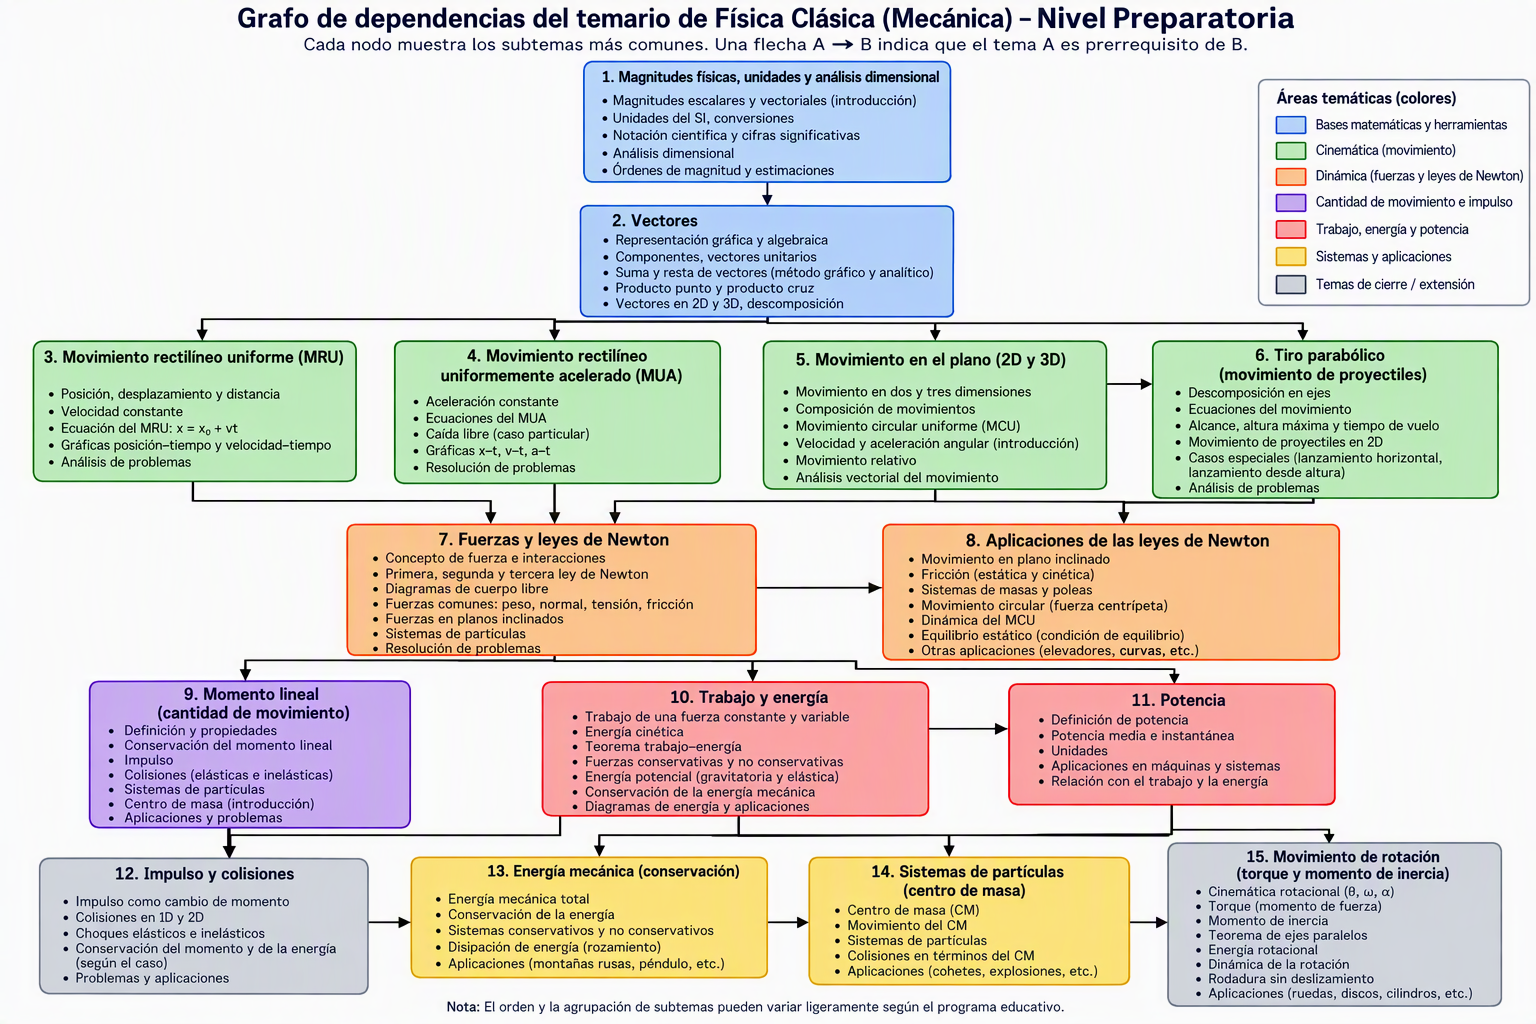
\includegraphics[width=\textwidth]{figuras/grafo_fisica.png}
\caption{Grafo de dependencias del temario de mecánica de bachillerato en el nivel de unidades.}
\label{fig:grafo}
\end{figure}

El modelo trata cada nodo como \emph{una habilidad con una sola memoria}, así que la granularidad importa:

\begin{itemize}
\item \textbf{Unidades} (15 nodos, 26 aristas). Son demasiado gruesas: «aplicaciones de las leyes de Newton» agrupa planos inclinados, poleas y curvas peraltadas, que no se olvidan en bloque.
\item \textbf{Subtemas} (168 nodos, 279 dependencias, 21 niveles de profundidad). Es el nivel de trabajo. Cada subtema es un procedimiento identificable («alcance horizontal», «fuerza de fricción cinética») para el que se pueden escribir problemas paramétricos. Las dependencias se anotaron a mano y están pendientes de validación docente.
\item \textbf{Prototipo} (13 subtemas de cinemática, de la conversión de unidades al alcance horizontal, con 33 plantillas).
\end{itemize}

La física de bachillerato es un buen primer dominio por cuatro razones: sus procedimientos son explícitos, el orden del temario es estable entre programas, cada problema admite infinitas instancias cambiando los datos y la mayoría de las respuestas son números con unidades que se califican automáticamente con una tolerancia.

\subsection{Arquitectura conceptual}

El sistema se describe como un conjunto de objetos matemáticos y funciones entre ellos, sin suponer lenguaje, base de datos ni plataforma. Separa cinco tipos de información que cambian por razones y a ritmos distintos:

\begin{enumerate}
\item \textbf{Dominio} $\Dom=(G,W,\Banco)$: el grafo $G$, la matriz $Q$ fraccional $W$ y el banco de plantillas $\Banco$. Lo editan los docentes.
\item \textbf{Parámetros del modelo} $\bm\theta$: cómo aprenden y olvidan los estudiantes en general. Se estiman con datos.
\item \textbf{Parámetros de la política} $\bm\varphi$: decisiones pedagógicas, como cuántos problemas por sesión o qué retención perseguir.
\item \textbf{Estado del estudiante} $\sigma$: lo que el sistema cree de cada estudiante. Cambia en cada intento.
\item \textbf{Historial} $\Hist$: lo que ocurrió (introducciones e intentos con su resultado). Solo crece.
\end{enumerate}

La decisión de diseño central es que \emph{el historial es la fuente de verdad y el estado es una consecuencia}: el estado se reconstruye en cualquier momento aplicando las reglas de actualización a los eventos en orden. Esto permite recalibrar $\bm\theta$ sin perder información y auditar cada decisión. La Figura~\ref{fig:arquitectura} muestra las siete funciones del sistema y cómo se conectan.

\begin{figure}[H]
\centering
\resizebox{\textwidth}{!}{%
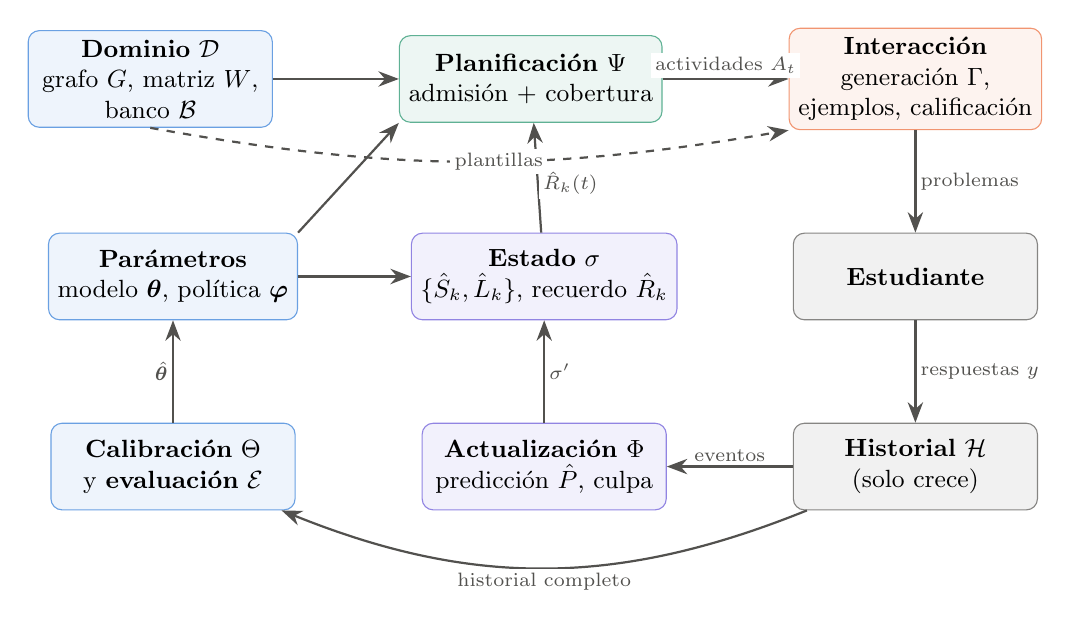
\begin{tikzpicture}[
  font=\small,
  caja/.style={draw=#1!70, fill=#1!8, rounded corners=4pt, minimum width=31mm, minimum height=11mm, align=center},
  fl/.style={-{Stealth[length=2.6mm]}, thick, gris},
  fll/.style={-{Stealth[length=2.6mm]}, thick, gris, dashed},
  lab/.style={font=\scriptsize, text=gris, fill=white, inner sep=1.5pt}
]
\node[caja=azul] (dom) {\textbf{Dominio} $\Dom$\\grafo $G$, matriz $W$,\\banco $\Banco$};
\node[caja=verde, right=16mm of dom] (plan) {\textbf{Planificación} $\Psi$\\admisión + cobertura};
\node[caja=naranja, right=16mm of plan] (int) {\textbf{Interacción}\\generación $\Gamma$,\\ejemplos, calificación};
\node[caja=gris, below=13mm of int] (est) {\textbf{Estudiante}};
\node[caja=gris, below=13mm of est] (hist) {\textbf{Historial} $\Hist$\\(solo crece)};
\node[caja=morado, left=16mm of hist] (act) {\textbf{Actualización} $\Phi$\\predicción $\hat P$, culpa};
\node[caja=morado, above=13mm of act] (sigma) {\textbf{Estado} $\sigma$\\$\{\Sh_k,\Lh_k\}$, recuerdo $\Rh_k$};
\node[caja=azul, left=16mm of act] (cal) {\textbf{Calibración} $\Theta$\\y \textbf{evaluación} $\mathcal E$};
\node[caja=azul, above=13mm of cal] (theta) {\textbf{Parámetros}\\modelo $\bm\theta$, política $\bm\varphi$};
\draw[fl] (dom) -- (plan);
\draw[fl] (plan) -- node[lab, above]{actividades $A_t$} (int);
\draw[fl] (int) -- node[lab, right]{problemas} (est);
\draw[fl] (est) -- node[lab, right]{respuestas $y$} (hist);
\draw[fl] (hist) -- node[lab, above]{eventos} (act);
\draw[fl] (act) -- node[lab, right]{$\sigma'$} (sigma);
\draw[fl] (sigma) -- node[lab, right, pos=0.45]{$\Rh_k(t)$} (plan);
\draw[fl] (hist) to[bend left=22] node[lab, below]{historial completo} (cal);
\draw[fl] (cal) -- node[lab, left]{$\hat{\bm\theta}$} (theta);
\draw[fl] (theta) -- (sigma);
\draw[fl] (theta.north east) -- (plan.south west);
\draw[fll] (dom.south) to[bend right=10] node[lab, pos=0.55]{plantillas} (int.south west);
\end{tikzpicture}}
\caption{Arquitectura conceptual. El ciclo de la derecha (planificación, interacción, historial y actualización) ocurre todos los días; el de la izquierda (calibración) ocurre cuando se acumulan datos suficientes.}
\label{fig:arquitectura}
\end{figure}

Cualquier implementación debe cumplir cinco invariantes:

\begin{invariante}[El estado es una reproducción del historial] No hay información en $\sigma$ que no provenga de $\Hist$ y $\bm\theta$.\end{invariante}
\begin{invariante}[Una actualización por habilidad por sesión] Si una habilidad ya se actualizó en la sesión del día (o se introdujo ese día), los intentos posteriores del mismo día no modifican su estabilidad.\end{invariante}
\begin{invariante}[Respeto al grafo] Una habilidad solo se introduce si sus prerrequisitos cumplen la condición de admisión~\eqref{eq:admision}.\end{invariante}
\begin{invariante}[Carga acotada] Al admitir habilidades nuevas, la carga esperada de repaso no excede una fracción $\rho$ de los problemas disponibles por sesión.\end{invariante}
\begin{invariante}[Instancias frescas] Cada intento usa una instancia nueva generada de una plantilla, para que el estudiante no pueda acertar recordando una respuesta.\end{invariante}

\subsection{El modelo}
\label{sec:modelo}

\paragraph{Notación.} $j$ y $k$ denotan habilidades (subtemas); $\Pre(k)$, los prerrequisitos directos de $k$; $t$, el tiempo en días. Para cada habilidad introducida, el estado guarda su estabilidad estimada $\Sh_k$ y el instante efectivo de su último repaso $\Lh_k$.

\paragraph{Matriz $Q$ fraccional.} Un problema del tipo $j$ ejercita por completo su tema y parcialmente sus prerrequisitos directos:
\begin{equation}
w_{jk}=\begin{cases}1 & k=j,\\ w_{\mathrm{pre}} & k\in\Pre(j),\\ 0 & \text{en otro caso,}\end{cases}
\qquad Q(j)=\{j\}\cup\Pre(j).
\label{eq:pesos}
\end{equation}
El valor $w_{\mathrm{pre}}=0.5$ es un supuesto inicial; con datos puede estimarse un peso por par.

\paragraph{Memoria.} El recuerdo estimado de la habilidad $k$ sigue la curva exponencial de \citet{tabibian2019}, con la estabilidad $\Sh_k=1/\hat n_k$ como variable:
\begin{equation}
\Rh_k(t)=\exp\!\left(-\frac{t-\Lh_k}{\Sh_k}\right).
\label{eq:memoria}
\end{equation}

\paragraph{Observación.} Resolver el problema exige recuperar todos sus componentes (modelo conjuntivo, como DINA), con descuido $s$ y adivinanza $g$ como en BKT:
\begin{equation}
\Pih_j(t)=\prod_{k\in Q(j)}\Rh_k(t)^{\,w_{jk}},\qquad
\hat P_j(t)=(1-s)\,\Pih_j(t)+g\,\bigl(1-\Pih_j(t)\bigr).
\label{eq:observacion}
\end{equation}
El peso en el exponente hace que un prerrequisito a medio olvidar estorbe menos que el tema principal a medio olvidar: con $\Rh=0.6$, la probabilidad de recuperarlo es $0.6$ si es el tema principal y $0.6^{0.5}=0.77$ si es prerrequisito.

\paragraph{Actualización tras un acierto.} La estabilidad de cada componente crece en proporción a lo olvidado, en línea con la hipótesis del esfuerzo de recuperación:
\begin{equation}
\Sh_k\leftarrow\Sh_k\,\bigl[1+w_{jk}\,G\,(1-\Rh_k)\bigr],\qquad k\in Q(j).
\label{eq:acierto}
\end{equation}
La ganancia es nula si $\Rh_k=1$: practicar justo después de la explicación no fortalece la memoria de largo plazo. Esta regla corrige la de la primera versión del protocolo, que premiaba la práctica concentrada. Si cada repaso ocurre cuando $\Rh=\rstar$, la estabilidad se multiplica por $1+G(1-\rstar)$ y los intervalos crecen geométricamente.

\paragraph{Salto del recuerdo.} Tras cualquier intento el estudiante ve la solución, así que el recuerdo sube. Es la ecuación de salto de \citet{tabibian2019}, $dm=(1-m)\,dN$, ponderada por el peso:
\begin{equation}
\Rh_k^{+}=\Rh_k+w_{jk}\bigl(1-\Rh_k\bigr),\qquad \Lh_k\leftarrow t+\Sh_k^{+}\,\ln\Rh_k^{+}.
\label{eq:salto}
\end{equation}
La segunda expresión elige el instante efectivo $\Lh_k$ que hace que~\eqref{eq:memoria}, con la estabilidad nueva, devuelva exactamente $\Rh_k^+$.

\paragraph{Culpa tras un fallo.} Tras un fallo no se observa qué componente falló. Por el teorema de Bayes, la probabilidad de que el componente $k$ no se haya recuperado, dado el fallo, es
\begin{equation}
b_k=\frac{\bigl(1-\Rh_k^{\,w_{jk}}\bigr)(1-g)}{\Pih_j\,s+\bigl(1-\Pih_j\bigr)(1-g)},
\label{eq:culpa}
\end{equation}
que con $s=g=0$ se reduce a $b_k=(1-\Rh_k^{\,w_{jk}})/(1-\Pih_j)$, la versión usada en la simulación. La culpa es mayor para el componente que tenía más probabilidad de fallar, y la versión completa la reduce cuando $\Pih_j\approx1$, porque un fallo así se explica mejor por un descuido.

\paragraph{Actualización tras un fallo.} Cada componente pierde estabilidad en proporción a su culpa, con un piso $\Smin$, y después se aplica el salto~\eqref{eq:salto}:
\begin{equation}
\Sh_k\leftarrow\max\bigl(\Smin,\ \Sh_k\,(1-\lambda\,b_k)\bigr),\qquad k\in Q(j).
\label{eq:fallo}
\end{equation}

\subsection{Planificación diaria}

\paragraph{Carga de repaso.} Una habilidad se repasa aproximadamente cada $\Sh_k\ln(1/\rstar)$ días, así que la carga esperada, en problemas por sesión, es
\begin{equation}
\Carga=\sum_{k\ \text{introducida}}\min\!\left(1,\ \frac{f}{\Sh_k\ln(1/\rstar)}\right),
\label{eq:carga}
\end{equation}
donde $f$ convierte días en sesiones ($f=7/5$ con cinco sesiones por semana). Como $\Sh_k$ crece con los repasos, la carga de una habilidad madura tiende a cero y el sistema libera espacio para temas nuevos.

\paragraph{Admisión.} Una habilidad $k$ no introducida es admisible el día $t$ si
\begin{equation}
\underbrace{\forall p\in\Pre(k):\ \Sh_p\ge\Slisto\ \text{y}\ \Rh_p(t)\ge\rstar}_{\text{sus bases están consolidadas}}
\quad\text{y}\quad
\underbrace{\Carga+m+1\le\rho\,U}_{\text{cabe en la sesión}},
\label{eq:admision}
\end{equation}
donde $U$ es el número de problemas por sesión y $m$ el de habilidades ya admitidas ese día. La primera condición es el borde externo de \citet{doignon1985} con «consolidado» en lugar de «sabido»; la segunda convierte la saturación de \citet{reddy2016} en una restricción explícita.

\paragraph{Cobertura submodular.} Sean $D$ las habilidades vencidas ($\Rh_k<\rstar$) y $\pi_k=1-\Rh_k$ su prioridad, que tiene la forma de la intensidad óptima $u^\ast\propto1-m$ de \citet{tabibian2019}. El planificador elige un conjunto $A$ de problemas que maximice
\begin{equation}
V(A)=\sum_{k\in D}\pi_k\Bigl[1-\prod_{j\in A}(1-w_{jk})\Bigr],
\label{eq:cobertura}
\end{equation}
la «masa vencida» que cubren. $V$ es monótona y submodular, así que el algoritmo voraz garantiza al menos $1-1/e$ del óptimo \citep{nemhauser1978}. El objetivo favorece los problemas integradores que repasan varias habilidades vencidas a la vez.

\paragraph{La sesión.} El plan del día se arma en tres fases: (1) cobertura voraz de las habilidades vencidas; (2) admisión de hasta $m_{\max}$ temas nuevos, cada uno con un ejemplo resuelto y práctica inicial, que ocupan $n_{\mathrm{intro}}$ lugares; (3) repasos adelantados de las habilidades con menor recuerdo, si sobran lugares.

\subsection{Estimación de parámetros}
\label{sec:estimacion}

Dado el historial, el estado antes de cada intento es una función determinista de $\bm\phi=(\Sh_0,G,\lambda)$. Por lo tanto, la predicción $\hat P_{in}(\bm\phi)$ del intento $n$ del estudiante $i$ es una función conocida de los parámetros, y se puede minimizar la log-verosimilitud negativa
\begin{equation}
\mathrm{NLL}(\bm\phi)=-\sum_i\sum_n\Bigl[y_{in}\ln\hat P_{in}(\bm\phi)+(1-y_{in})\ln\bigl(1-\hat P_{in}(\bm\phi)\bigr)\Bigr]
\label{eq:nll}
\end{equation}
con un método sin derivadas, como Nelder--Mead, sobre $(\ln\Sh_0,\ \ln G,\ \operatorname{logit}\lambda)$. Para que los parámetros sean identificables, el piloto debe repasar con intervalos variados y no con la política final. Con datos reales se considerará un modelo jerárquico con efectos por estudiante y por subtema, $\ln\Sh_{0,ik}=\mu_k+\alpha_i$, estimado de forma bayesiana.

\subsection{Resumen de parámetros}

\begin{table}[H]
\centering\small
\caption{Parámetros del sistema. Los del modelo describen a los estudiantes en general; los de la política son decisiones pedagógicas. Los valores estimados provienen del piloto simulado y se reestimarán con datos reales.}
\label{tab:parametros}
\begin{tabularx}{\textwidth}{@{}llllY@{}}
\toprule
& \textbf{Símbolo} & \textbf{Valor} & \textbf{Origen} & \textbf{Interpretación} \\
\midrule
\multirow{7}{*}{Modelo}
& $\Sh_0$ & 8.2 d & estimado & estabilidad inicial de un tema recién visto \\
& $G$ & 7.2 & estimado & ganancia por acierto \\
& $\lambda$ & 0.13 & estimado & severidad del fallo \\
& $s$ & 0.05 & fijado & descuido \\
& $g$ & 0.02 & fijado & adivinanza (problemas abiertos) \\
& $w_{\mathrm{pre}}$ & 0.5 & fijado & peso de un prerrequisito \\
& $\Smin$ & 0.2 d & fijado & piso de estabilidad \\
\midrule
\multirow{7}{*}{Política}
& $\rstar$ & 0.7 & diseño & retención objetivo \\
& $r_{\min}$ & 0.6 & diseño & recuerdo mínimo de los componentes de apoyo \\
& $\Slisto$ & 7--12 d & diseño & firmeza mínima de un prerrequisito \\
& $\rho$ & 0.8 & diseño & fracción máxima de la sesión para repasos \\
& $U$ & 5--10 & diseño & problemas por sesión \\
& $n_{\mathrm{intro}}$ & 2 & diseño & lugares que ocupa un tema nuevo \\
& $m_{\max}$ & 2--3 & diseño & temas nuevos por día \\
\bottomrule
\end{tabularx}
\end{table}

%=====================================================================
\section{Avances y resultados preliminares}
\label{sec:avances}
%=====================================================================

\subsection{Simulador}

Evaluar el planificador con el mismo modelo con el que se generan los datos garantizaría el éxito por construcción. Por eso el simulador separa la \emph{verdad} (cómo aprende y olvida el estudiante simulado, que el planificador nunca ve) del \emph{modelo}, y especifica mal el segundo respecto a la primera a propósito (Tabla~\ref{tab:verdad}).

\begin{table}[H]
\centering\small
\caption{Diferencias deliberadas entre el estudiante simulado y el modelo del planificador.}
\label{tab:verdad}
\begin{tabularx}{\textwidth}{@{}lYY@{}}
\toprule
& \textbf{Verdad (estudiante simulado)} & \textbf{Modelo (planificador)} \\
\midrule
Olvido & ley de potencia & exponencial~\eqref{eq:memoria} \\
Ganancia por acierto & tipo FSRS, con rendimientos decrecientes & $G(1-\Rh)$~\eqref{eq:acierto} \\
Fallo & lapso solo en los componentes que no se recuperaron & culpa repartida~\eqref{eq:culpa} \\
Bases débiles & escenario A: efecto leve; B: efecto persistente & solo la compuerta de admisión \\
Diferencias entre estudiantes & habilidad latente $\theta_i\sim N(0,0.35^2)$ & ninguna \\
\bottomrule
\end{tabularx}
\end{table}

El curso simulado dura 12 semanas con 5 sesiones por semana. La métrica principal es la probabilidad media, sobre todas las habilidades del grafo, de que el estudiante resuelva un problema nuevo de cada una 30 días después de la última sesión, sin práctica intermedia. Un tema no introducido vale $g=0.02$, así que la métrica premia tanto la retención como la cobertura. Cada política se aplica a los mismos 300 estudiantes simulados y las diferencias se reportan pareadas. Los parámetros del modelo se estiman en cada escenario con un piloto simulado de 100 estudiantes distintos.

Las políticas comparadas son: el sistema propuesto (con $\rstar=0.7$ y $\rstar=0.9$) y sus ablaciones; Anki SM-2 con una tarjeta por tema y límite de temas nuevos por día; el libro bloqueado (un tema tras otro, sin repaso); y el libro con repaso acumulativo (2 de los $U$ problemas son de temas anteriores al azar).

\subsection{Resultados}

\paragraph{Grafo de unidades.} Con 15 unidades y 60 sesiones hay tiempo de sobra y todas las políticas introducen todo el temario. Cualquier política con repaso espaciado supera al libro bloqueado por 0.28--0.29, pero el sistema propuesto (0.743 en el escenario A y 0.714 en el B) no supera a Anki SM-2 (0.749 y 0.722). Solo con un presupuesto escaso ($U=4$) aparece una ventaja pequeña.

\paragraph{Grafo de subtemas.} Con 168 subtemas ninguna política adaptativa alcanza a introducirlos todos, y el resultado cambia (Tabla~\ref{tab:subtemas} y Figura~\ref{fig:barras}). El sistema propuesto supera a Anki por $+0.090$ (A) y $+0.047$ (B), y la ventaja se mantiene con $U$ entre 6 y 14. El mecanismo es la cobertura: Anki acumula repasos vencidos y deja de introducir temas (71 frente a 106 en A). En cambio, Anki deja más subtemas con probabilidad de acierto de al menos 0.8, de modo que, por tema introducido, retiene más. El crédito a prerrequisitos aporta $+0.014$ en A, la compuerta $+0.015$ en B y la culpa bayesiana entre $+0.002$ y $+0.004$. Quitar el control de carga mejora la métrica en $+0.027$, a costa de introducir temas con menos retención: en esta métrica, el control de carga es conservador.

\begin{table}[H]
\centering\small
\caption{Grafo de 168 subtemas ($U=10$, $m_{\max}=3$). Examen diferido (media por estudiante), diferencia pareada respecto al propuesto y temas introducidos. Los IC del 95\,\% de las diferencias son de aproximadamente $\pm0.002$.}
\label{tab:subtemas}
\setlength{\tabcolsep}{3.5pt}
\begin{tabular}{@{}lcccccc@{}}
\toprule
& \multicolumn{3}{c}{A: efecto leve} & \multicolumn{3}{c}{B: efecto persistente} \\
\cmidrule(lr){2-4}\cmidrule(lr){5-7}
Política & Examen & $\Delta$ & Temas & Examen & $\Delta$ & Temas \\
\midrule
Propuesto ($\rstar=0.7$) & 0.370 & --- & 106 & 0.285 & --- & 79 \\
Propuesto ($\rstar=0.9$) & 0.239 & $-0.131$ & 56 & 0.189 & $-0.097$ & 42 \\
\quad sin crédito a prerrequisitos & 0.355 & $-0.014$ & 98 & 0.282 & $-0.003$ & 74 \\
\quad sin culpa bayesiana & 0.366 & $-0.004$ & 103 & 0.283 & $-0.002$ & 78 \\
\quad sin control de carga & 0.397 & $+0.027$ & 134 & 0.312 & $+0.026$ & 101 \\
\quad sin compuerta & 0.372 & $+0.002$ & 108 & 0.270 & $-0.015$ & 79 \\
Anki SM-2 & 0.280 & $-0.090$ & 71 & 0.239 & $-0.047$ & 63 \\
Libro + repaso acumulativo & 0.275 & $-0.095$ & 168 & 0.144 & $-0.142$ & 168 \\
Libro bloqueado & 0.167 & $-0.203$ & 168 & 0.078 & $-0.207$ & 168 \\
\bottomrule
\end{tabular}
\end{table}

\begin{figure}[H]
\centering
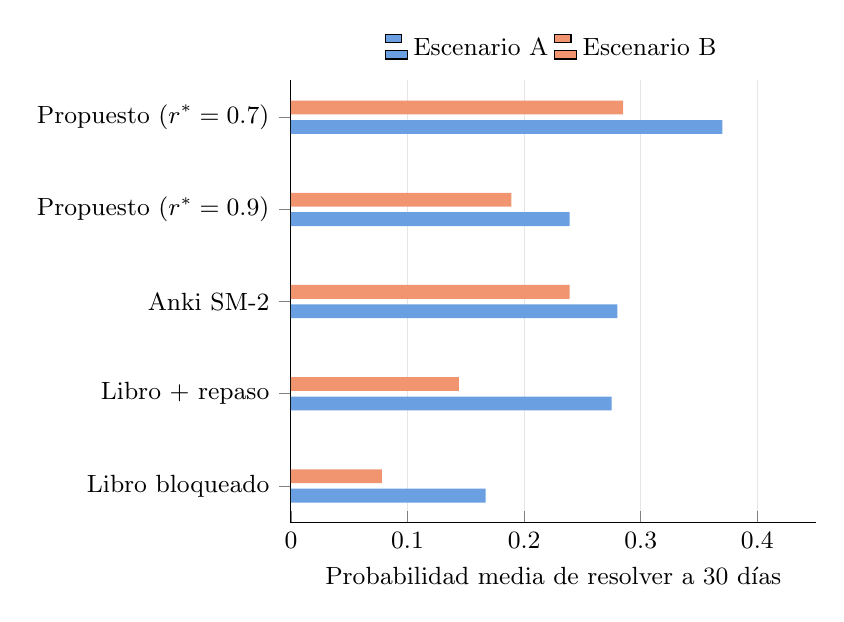
\begin{tikzpicture}
\begin{axis}[
  xbar, width=0.68\textwidth, height=7.2cm,
  bar width=5pt, enlarge y limits=0.1,
  xmin=0, xmax=0.45,
  xlabel={Probabilidad media de resolver a 30 días},
  symbolic y coords={lb,lr,anki,p9,p7},
  yticklabels={Libro bloqueado,Libro + repaso,Anki SM-2,Propuesto ($r^*=0.9$),Propuesto ($r^*=0.7$)},
  ytick=data, y tick label style={font=\small}, x tick label style={font=\small,/pgf/number format/fixed},
  label style={font=\small},
  legend style={at={(0.5,1.02)},anchor=south,legend columns=2,font=\small,draw=none},
  axis lines*=left, xmajorgrids, grid style={gray!20},
]
\addplot[fill=azul!70, draw=none] coordinates {(0.167,lb) (0.275,lr) (0.280,anki) (0.239,p9) (0.370,p7)};
\addplot[fill=naranja!70, draw=none] coordinates {(0.078,lb) (0.144,lr) (0.239,anki) (0.189,p9) (0.285,p7)};
\legend{Escenario A, Escenario B}
\end{axis}
\end{tikzpicture}
\caption{Examen diferido en el grafo de 168 subtemas, por política y escenario (datos de la Tabla~\ref{tab:subtemas}).}
\label{fig:barras}
\end{figure}

\paragraph{La estructura del grafo importa.} Como control, se repitió la simulación sustituyendo las dependencias explícitas por cadenas lineales (cada unidad como una fila de subtemas en orden). En el escenario A la ventaja sobre Anki baja de $+0.090$ a $+0.012$; en el B el sistema propuesto cae a 0.124 y queda $0.115$ por debajo de Anki, porque con 103 niveles de profundidad solo hay un tema admisible a la vez. Un grafo con dependencias falsas castiga justamente al sistema que lo respeta. Por eso la validación docente del grafo es parte de la metodología y no un detalle.

\paragraph{Calidad de las predicciones.} Fuera de muestra, el modelo exponencial obtiene un AUC de 0.67 y un puntaje de Brier de 0.17--0.18 en el grafo de subtemas, y sobreestima la probabilidad de acierto en el rango medio. Es lo esperable, porque la verdad usa olvido de ley de potencia y lapsos ocultos. Aun así, el planificador funciona razonablemente bien, y la calibración será el diagnóstico para detectar la mala especificación con datos reales.

\subsection{Prototipo}

El prototipo es una aplicación web escrita en HTML, CSS y JavaScript, sin servidor, con dos paneles: a la izquierda, lo que ve el estudiante (problema, respuesta, solución resuelta); a la derecha, lo que hace el sistema (estado de cada habilidad, predicción, actualización de parámetros y bitácora de eventos). Un botón adelanta el reloj un día para observar el olvido y la planificación. Usa el subgrafo de 13 subtemas de cinemática y 33 plantillas paramétricas almacenadas en archivos JSON, con un evaluador seguro de expresiones para generar instancias y calcular respuestas. El prototipo implementa las ecuaciones~\eqref{eq:pesos}--\eqref{eq:cobertura}; todavía no implementa la calibración ni reconstruye el estado a partir del historial.

\subsection{Lecciones para la segunda mitad de la tesis}

\begin{enumerate}
\item La ventaja del modelo depende de dos condiciones del dominio: un grafo de grano fino con presupuesto de práctica escaso y dependencias fieles. Ambas se verificarán con datos reales.
\item El efecto más grande y robusto es espaciar frente a no espaciar ($+0.20$ a $+0.29$). Entre políticas espaciadas las diferencias son menores, lo que determina el tamaño de muestra del experimento.
\item El valor $\rstar=0.7$ se eligió tras un barrido preliminar con la verdad simulada. En la tesis se fijará con un procedimiento que no use la verdad, por ejemplo optimizándolo en simulación con el modelo ajustado al piloto.
\item La métrica favorece la cobertura. Un $\rstar$ bajo implica más fallos durante la práctica, con posibles costos de motivación que la simulación no modela y que el experimento debe registrar.
\end{enumerate}

%=====================================================================
\section{Metodología}
\label{sec:metodologia}
%=====================================================================

El proyecto sigue un enfoque de investigación basada en diseño (\emph{design-based research}): el sistema se desarrolla en ciclos de diseño, evaluación y refinamiento. A diferencia de la versión anterior del protocolo, la evaluación se escalona en tres niveles de evidencia, de menor a mayor costo: simulación, piloto de calibración y experimento en aula. Cada nivel decide si vale la pena pasar al siguiente. La investigación se organiza en seis fases (Figura~\ref{fig:metodologia}).

\begin{figure}[H]
\centering
\resizebox{\textwidth}{!}{%
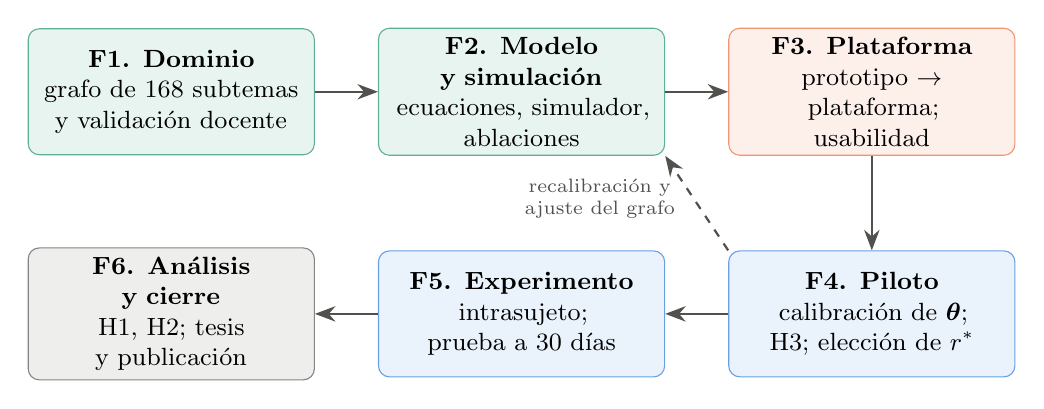
\begin{tikzpicture}[
  font=\small,
  fase/.style={draw=#1!70, fill=#1!10, rounded corners=4pt, minimum width=36mm, minimum height=16mm, align=center, text width=34mm},
  fl/.style={-{Stealth[length=2.6mm]}, thick, gris},
  lab/.style={font=\scriptsize, text=gris, align=center}
]
\node[fase=verde] (f1) {\textbf{F1. Dominio}\\grafo de 168 subtemas\\y validación docente};
\node[fase=verde, right=8mm of f1] (f2) {\textbf{F2. Modelo y simulación}\\ecuaciones, simulador,\\ablaciones};
\node[fase=naranja, right=8mm of f2] (f3) {\textbf{F3. Plataforma}\\prototipo $\to$ plataforma;\\usabilidad};
\node[fase=azul, below=12mm of f3] (f4) {\textbf{F4. Piloto}\\calibración de $\bm\theta$;\\H3; elección de $\rstar$};
\node[fase=azul, left=8mm of f4] (f5) {\textbf{F5. Experimento}\\intrasujeto;\\prueba a 30 días};
\node[fase=gris, left=8mm of f5] (f6) {\textbf{F6. Análisis}\\\textbf{y cierre}\\H1, H2; tesis\\y publicación};
\draw[fl] (f1) -- (f2);
\draw[fl] (f2) -- (f3);
\draw[fl] (f3) -- (f4);
\draw[fl] (f4) -- (f5);
\draw[fl] (f5) -- (f6);
\draw[fl, dashed] (f4.north west) -- node[lab, left=3pt, pos=0.55]{recalibración y\\ajuste del grafo} (f2.south east);
\end{tikzpicture}}
\caption{Fases de la metodología. Verde: concluidas o en curso; naranja: en curso; azul y gris: por realizar. La flecha punteada indica el ciclo de refinamiento.}
\label{fig:metodologia}
\end{figure}

\subsection{Fase 1: dominio y grafo de habilidades (febrero de 2026 a marzo de 2027)}

\begin{itemize}
\item \textbf{Actividades:} revisión de la literatura; construcción del grafo de mecánica en dos niveles (15 unidades con 26 aristas; 168 subtemas con 279 dependencias); conciliación entre la figura del temario y la lista formal de aristas; validación del grafo de subtemas con docentes.
\item \textbf{Instrumentos:} matriz de revisión de literatura; formato de validación en el que al menos tres docentes de física de bachillerato marcan, para cada dependencia, si es necesaria, útil o falsa, y proponen dependencias faltantes. El acuerdo entre docentes se reportará con el coeficiente kappa de Fleiss.
\item \textbf{Estado:} grafo construido; validación docente pendiente.
\item \textbf{Entregable:} grafo validado y documentado en formato de datos.
\end{itemize}

\subsection{Fase 2: modelo y evaluación por simulación (marzo de 2026 a enero de 2027)}

\begin{itemize}
\item \textbf{Actividades:} formulación del modelo (sección~\ref{sec:modelo}); simulador Monte Carlo con estudiante mal especificado; comparación contra políticas de referencia; ablaciones y análisis de sensibilidad; control estructural con cadenas lineales.
\item \textbf{Pendiente:} implementar la culpa completa~\eqref{eq:culpa} en el simulador; fijar $\rstar$ con un procedimiento que no use la verdad; repetir los resultados con el grafo validado.
\item \textbf{Estado:} concluida en lo esencial (sección~\ref{sec:avances}).
\item \textbf{Entregables:} dos documentos técnicos (modelo y simulación; arquitectura y ecuaciones) y el código del simulador.
\end{itemize}

\subsection{Fase 3: plataforma web (octubre de 2026 a marzo de 2027)}

\begin{itemize}
\item \textbf{Actividades:} extender el prototipo a una plataforma con cuentas de estudiante y docente; historial de eventos como fuente de verdad y estado reconstruible; banco de plantillas paramétricas con al menos dos plantillas por subtema incluido en el piloto y el experimento; política de referencia (SM-2 o FSRS con límite de temas nuevos) implementada en la misma plataforma, para que ambas condiciones tengan la misma interfaz; vista docente.
\item \textbf{Instrumentos:} pruebas de usabilidad con al menos 10 estudiantes, escala SUS \citep{brooke1996}, registro de errores y pruebas automatizadas que comparen el estado reconstruido con el estado incremental.
\item \textbf{Estado:} prototipo funcional con 13 subtemas y 33 plantillas.
\item \textbf{Entregable:} plataforma desplegada en un entorno de prueba accesible desde computadoras y teléfonos.
\end{itemize}

\subsection{Fase 4: piloto de calibración (marzo a mayo de 2027)}

\begin{itemize}
\item \textbf{Diseño:} entre 30 y 40 estudiantes practican durante 4 a 6 semanas un subconjunto del grafo (por ejemplo, cinemática). Los temas se introducen en el orden del temario y los repasos se programan con \emph{intervalos aleatorios}, no con la política final, para que los parámetros sean identificables (sección~\ref{sec:estimacion}).
\item \textbf{Análisis:} estimación de $(\Sh_0,G,\lambda)$ por máxima verosimilitud~\eqref{eq:nll} y, si los datos lo permiten, de $s$, $g$ y del modelo jerárquico; calibración fuera de muestra (AUC, Brier y curva de calibración); prueba de la hipótesis~\ref{h:modelo} comparando $w_{\mathrm{pre}}=0.5$ contra $w_{\mathrm{pre}}=0$ y comparación de las formas exponencial y de potencia, ambas por log-verosimilitud con validación cruzada por estudiante.
\item \textbf{Decisiones que alimenta:} parámetros del modelo para el experimento; elección de $\rstar$ en simulación con el modelo ajustado; ajustes al grafo si alguna dependencia no se sostiene en los datos.
\item \textbf{Entregable:} informe de calibración y parámetros congelados para el experimento.
\end{itemize}

\subsection{Fase 5: experimento en aula (agosto a diciembre de 2027)}

\begin{itemize}
\item \textbf{Diseño:} intrasujeto y contrabalanceado, al estilo de \citet{lindsey2014}. Los subtemas del experimento se dividen en dos conjuntos equivalentes en tamaño, profundidad y dificultad, formados por ramas del grafo que no dependen entre sí; los prerrequisitos comunes (magnitudes, vectores) se enseñan a todos por igual antes de empezar. Cada estudiante practica un conjunto con el sistema propuesto y el otro con la política de referencia; la asignación de conjuntos a políticas se contrabalancea entre estudiantes. Ambas políticas reciben el mismo número de problemas por sesión, así que el tiempo de práctica queda igualado.
\item \textbf{Participantes:} estudiantes de bachillerato de al menos dos escuelas públicas del Estado de México. Con diferencias pareadas, $\alpha=0.05$ y potencia de 0.8, el tamaño de muestra necesario es $n\approx7.85/d_z^2$: 32 estudiantes para un efecto $d_z=0.5$ y 88 para $d_z=0.3$. La meta es reclutar al menos 90 estudiantes, previendo bajas.
\item \textbf{Intervención:} entre 8 y 12 semanas, según el calendario escolar, con sesiones cortas de 15 a 20 minutos, cinco días por semana.
\item \textbf{Instrumentos:}
\begin{itemize}
\item \emph{prueba diagnóstica} al inicio, para verificar que los dos conjuntos parten del mismo nivel;
\item \emph{prueba diferida} 30 días después de la última sesión, con problemas nuevos de cada subtema de ambos conjuntos, generados de plantillas que no se usaron durante la práctica;
\item \emph{registros de la plataforma}: intentos, aciertos, temas introducidos, sesiones completadas y tiempo por problema;
\item \emph{encuesta final}: escala SUS, carga percibida y preferencias, con preguntas abiertas.
\end{itemize}
\item \textbf{Análisis:} la hipótesis~\ref{h:principal} se prueba con un modelo logístico mixto de los aciertos en la prueba diferida, con la condición como efecto fijo y el estudiante y el subtema como efectos aleatorios; se reportan el tamaño del efecto y su intervalo de confianza. La hipótesis~\ref{h:mecanismo} se evalúa descomponiendo la diferencia en cobertura (subtemas introducidos) y retención por subtema introducido. El análisis se prerregistrará antes de recolectar los datos.
\item \textbf{Análisis cualitativo:} análisis temático de las respuestas abiertas y de entrevistas breves con un subgrupo de estudiantes ($n\approx10$) y con los docentes participantes.
\end{itemize}

\subsection{Fase 6: análisis, refinamiento y cierre (noviembre de 2027 a enero de 2028)}

\begin{itemize}
\item \textbf{Actividades:} análisis integrado de los resultados; recalibración del modelo con todos los datos; comparación entre las predicciones de la simulación y lo observado; redacción de la tesis; envío de un artículo a un congreso o revista del área (por ejemplo, \emph{Educational Data Mining} o \emph{Artificial Intelligence in Education}).
\item \textbf{Entregables:} tesis, repositorio con el código del simulador y de la plataforma, datos anonimizados (si las autorizaciones lo permiten) y guía de uso para docentes.
\end{itemize}

\subsection{Riesgos y mitigación}

\begin{table}[H]
\centering\small
\caption{Riesgos principales y cómo se mitigan.}
\label{tab:riesgos}
\begin{tabularx}{\textwidth}{@{}P{4.2cm}Y@{}}
\toprule
\textbf{Riesgo} & \textbf{Mitigación} \\
\midrule
Dependencias falsas en el grafo & Validación docente (fase 1) y revisión con los datos del piloto (fase 4); la simulación ya cuantificó el costo de este error \\
Parámetros no identificables & Piloto con intervalos aleatorios; parámetros fijos ($s$, $g$) si los datos no alcanzan \\
Baja adherencia & Sesiones cortas dentro del horario escolar, acordadas con los docentes \\
Acceso limitado a escuelas & Contacto con las escuelas desde la fase 3; una escuela adicional como respaldo \\
Muestra menor a la planeada & Reportar el efecto mínimo detectable con la muestra obtenida; el diseño intrasujeto reduce el tamaño necesario \\
Contaminación entre condiciones & Conjuntos de subtemas en ramas independientes del grafo; prerrequisitos comunes enseñados antes del experimento \\
\bottomrule
\end{tabularx}
\end{table}

\subsection{Consideraciones éticas}

El proyecto se someterá al comité de ética de la institución antes del piloto. Como los participantes son en su mayoría menores de edad, sus padres o tutores firmarán un consentimiento informado y cada estudiante dará su asentimiento. La participación no afectará las calificaciones escolares y cualquier estudiante podrá retirarse sin consecuencias. Los datos se guardarán con identificadores seudónimos y solo el equipo de investigación tendrá acceso a la correspondencia con los nombres. El diseño intrasujeto tiene además una ventaja ética: todos los estudiantes reciben las dos formas de práctica espaciada y ninguno queda en una condición sin repaso.

%=====================================================================
\section{Cronograma de actividades}
\label{sec:cronograma}
%=====================================================================

La Tabla~\ref{tab:cronograma} presenta el cronograma por semestre. S1 corresponde a febrero--julio de 2026, S2 a agosto de 2026--enero de 2027, S3 a febrero--julio de 2027 y S4 a agosto de 2027--enero de 2028. Las marcas \textbf{X} indican actividades concluidas y las marcas $\bullet$, actividades en curso o por realizar.

\begin{table}[H]
\centering\small
\caption{Cronograma de actividades por semestre.}
\label{tab:cronograma}
\begin{tabular}{@{}P{8.6cm}cccc@{}}
\toprule
\textbf{Actividad} & \textbf{S1} & \textbf{S2} & \textbf{S3} & \textbf{S4} \\
\midrule
\textbf{Fase 1: dominio y grafo} & & & & \\
\quad Revisión de literatura & X & X & $\bullet$ & \\
\quad Grafo de unidades y de subtemas & X & X & & \\
\quad Validación docente del grafo & & $\bullet$ & $\bullet$ & \\
\midrule
\textbf{Fase 2: modelo y simulación} & & & & \\
\quad Formulación del modelo & X & X & & \\
\quad Simulador, comparación y ablaciones & & X & & \\
\quad Ajustes pendientes del modelo y del simulador & & $\bullet$ & $\bullet$ & \\
\midrule
\textbf{Fase 3: plataforma} & & & & \\
\quad Prototipo funcional & & X & & \\
\quad Plataforma y banco de plantillas & & $\bullet$ & $\bullet$ & \\
\quad Pruebas de usabilidad & & & $\bullet$ & \\
\midrule
\textbf{Fase 4: piloto de calibración} & & & & \\
\quad Comité de ética y consentimientos & & $\bullet$ & $\bullet$ & \\
\quad Piloto y estimación de parámetros & & & $\bullet$ & \\
\midrule
\textbf{Fase 5: experimento en aula} & & & & \\
\quad Prerregistro y prueba diagnóstica & & & $\bullet$ & $\bullet$ \\
\quad Intervención & & & & $\bullet$ \\
\quad Prueba diferida a 30 días & & & & $\bullet$ \\
\midrule
\textbf{Fase 6: análisis y cierre} & & & & \\
\quad Análisis cuantitativo y cualitativo & & & & $\bullet$ \\
\quad Redacción de la tesis & & & $\bullet$ & $\bullet$ \\
\quad Publicación y difusión & & & & $\bullet$ \\
\bottomrule
\end{tabular}
\end{table}

%=====================================================================
% Referencias
%=====================================================================
\begin{thebibliography}{99}
\small

\bibitem[{Arthur et~al.(1998)}]{arthur1998}
Arthur, W., Bennett, W., Stanush, P.~L. y McNelly, T.~L. (1998).
\newblock Factors that influence skill decay and retention: A quantitative review and analysis.
\newblock \emph{Human Performance}, 11(1):57--101.

\bibitem[{Barzagar~Nazari y Ebersbach(2019)}]{barzagar2019}
Barzagar~Nazari, K. y Ebersbach, M. (2019).
\newblock Distributing mathematical practice of third and seventh graders: Applicability of the spacing effect in the classroom.
\newblock \emph{Applied Cognitive Psychology}, 33(2):288--298.

\bibitem[{Brooke(1996)}]{brooke1996}
Brooke, J. (1996).
\newblock SUS: A ``quick and dirty'' usability scale.
\newblock En Jordan, P.~W., Thomas, B., Weerdmeester, B.~A. y McClelland, I.~L. (eds.), \emph{Usability Evaluation in Industry}, pp.~189--194. Taylor \& Francis.

\bibitem[{Cen et~al.(2006)}]{cen2006}
Cen, H., Koedinger, K. y Junker, B. (2006).
\newblock Learning factors analysis: A general method for cognitive model evaluation and improvement.
\newblock En \emph{Intelligent Tutoring Systems (ITS 2006)}, pp.~164--175. Springer.

\bibitem[{Cepeda et~al.(2006)}]{cepeda2006}
Cepeda, N.~J., Pashler, H., Vul, E., Wixted, J.~T. y Rohrer, D. (2006).
\newblock Distributed practice in verbal recall tasks: A review and quantitative synthesis.
\newblock \emph{Psychological Bulletin}, 132(3):354--380.

\bibitem[{Cepeda et~al.(2008)}]{cepeda2008}
Cepeda, N.~J., Vul, E., Rohrer, D., Wixted, J.~T. y Pashler, H. (2008).
\newblock Spacing effects in learning: A temporal ridgeline of optimal retention.
\newblock \emph{Psychological Science}, 19(11):1095--1102.

\bibitem[{Choffin et~al.(2019)}]{choffin2019}
Choffin, B., Popineau, F., Bourda, Y. y Vie, J.-J. (2019).
\newblock DAS3H: Modeling student learning and forgetting for optimally scheduling distributed practice of skills.
\newblock En \emph{Proceedings of the 12th International Conference on Educational Data Mining (EDM 2019)}, pp.~29--38.

\bibitem[{Choffin et~al.(2021)}]{choffin2021}
Choffin, B., Popineau, F. y Bourda, Y. (2021).
\newblock Extending adaptive spacing heuristics to multi-skill items.
\newblock \emph{Journal of Educational Data Mining}, 13(3):69--102.

\bibitem[{Corbett y Anderson(1994)}]{corbett1994}
Corbett, A.~T. y Anderson, J.~R. (1994).
\newblock Knowledge tracing: Modeling the acquisition of procedural knowledge.
\newblock \emph{User Modeling and User-Adapted Interaction}, 4(4):253--278.

\bibitem[{de~la Torre(2011)}]{delatorre2011}
de~la Torre, J. (2011).
\newblock The generalized DINA model framework.
\newblock \emph{Psychometrika}, 76(2):179--199.

\bibitem[{Doignon y Falmagne(1985)}]{doignon1985}
Doignon, J.-P. y Falmagne, J.-C. (1985).
\newblock Spaces for the assessment of knowledge.
\newblock \emph{International Journal of Man-Machine Studies}, 23(2):175--196.

\bibitem[{Gilbert et~al.(2023)}]{gilbert2023}
Gilbert, M.~M., Frommeyer, T.~C., Brittain, G.~V., Stewart, N.~A., Turner, T.~M., Stolfi, A. y Parmelee, D. (2023).
\newblock A cohort study assessing the impact of Anki as a spaced repetition tool on academic performance in medical school.
\newblock \emph{Medical Science Educator}, 33(4):955--962.

\bibitem[{Hunziker et~al.(2019)}]{hunziker2019}
Hunziker, A., Chen, Y., Mac~Aodha, O., Gomez-Rodriguez, M., Krause, A., Perona, P., Yue, Y. y Singla, A. (2019).
\newblock Teaching multiple concepts to a forgetful learner.
\newblock En \emph{Advances in Neural Information Processing Systems 32 (NeurIPS 2019)}.

\bibitem[{Jape et~al.(2022)}]{jape2022}
Jape, D., Zhou, J. y Bullock, S. (2022).
\newblock A spaced-repetition approach to enhance medical student learning and engagement in medical pharmacology.
\newblock \emph{BMC Medical Education}, 22:337.

\bibitem[{Junker y Sijtsma(2001)}]{junker2001}
Junker, B.~W. y Sijtsma, K. (2001).
\newblock Cognitive assessment models with few assumptions, and connections with nonparametric item response theory.
\newblock \emph{Applied Psychological Measurement}, 25(3):258--272.

\bibitem[{Kang(2016)}]{kang2016}
Kang, S.~H.~K. (2016).
\newblock Spaced repetition promotes efficient and effective learning: Policy implications for instruction.
\newblock \emph{Policy Insights from the Behavioral and Brain Sciences}, 3(1):12--19.

\bibitem[{Koedinger et~al.(2012)}]{koedinger2012}
Koedinger, K.~R., Corbett, A.~T. y Perfetti, C. (2012).
\newblock The Knowledge-Learning-Instruction framework: Bridging the science-practice chasm to enhance robust student learning.
\newblock \emph{Cognitive Science}, 36(5):757--798.

\bibitem[{Lindsey et~al.(2014)}]{lindsey2014}
Lindsey, R.~V., Shroyer, J.~D., Pashler, H. y Mozer, M.~C. (2014).
\newblock Improving students' long-term knowledge retention through personalized review.
\newblock \emph{Psychological Science}, 25(3):639--647.

\bibitem[{Mostrady et~al.(2025)}]{mostrady2025}
Mostrady, A., Sanchez-Lopez, E. y Gonzalez-Sanchez, A.~F. (2025).
\newblock Microlearning: A review of concept, technological platforms, and effectiveness.
\newblock \emph{Acta Pedagogia Asiana}, 4(1):33--42.

\bibitem[{Nemhauser et~al.(1978)}]{nemhauser1978}
Nemhauser, G.~L., Wolsey, L.~A. y Fisher, M.~L. (1978).
\newblock An analysis of approximations for maximizing submodular set functions---I.
\newblock \emph{Mathematical Programming}, 14(1):265--294.

\bibitem[{Pavlik et~al.(2009)}]{pavlik2009}
Pavlik, P.~I., Cen, H. y Koedinger, K.~R. (2009).
\newblock Performance factors analysis: A new alternative to knowledge tracing.
\newblock En \emph{Artificial Intelligence in Education (AIED 2009)}, pp.~531--538. IOS Press.

\bibitem[{Price et~al.(2025)}]{price2025}
Price, D.~W., Wang, T., O'Neill, T.~R., Morgan, Z.~J., Chodavarapu, P., Bazemore, A., Peterson, L.~E. y Newton, W.~P. (2025).
\newblock The effect of spaced repetition on learning and knowledge transfer in a large cohort of practicing physicians.
\newblock \emph{Academic Medicine}, 100(1):94--102.

\bibitem[{Pyc y Rawson(2009)}]{pyc2009}
Pyc, M.~A. y Rawson, K.~A. (2009).
\newblock Testing the retrieval effort hypothesis: Does greater difficulty correctly recalling information lead to higher levels of memory?
\newblock \emph{Journal of Memory and Language}, 60(4):437--447.

\bibitem[{Reddy et~al.(2016)}]{reddy2016}
Reddy, S., Labutov, I., Banerjee, S. y Joachims, T. (2016).
\newblock Unbounded human learning: Optimal scheduling for spaced repetition.
\newblock En \emph{Proceedings of the 22nd ACM SIGKDD International Conference on Knowledge Discovery and Data Mining}, pp.~1815--1824.

\bibitem[{Rohrer et~al.(2015)}]{rohrer2015}
Rohrer, D., Dedrick, R.~F. y Stershic, S. (2015).
\newblock Interleaved practice improves mathematics learning.
\newblock \emph{Journal of Educational Psychology}, 107(3):900--908.

\bibitem[{Rohrer y Taylor(2007)}]{rohrer2007}
Rohrer, D. y Taylor, K. (2007).
\newblock The shuffling of mathematics problems improves learning.
\newblock \emph{Instructional Science}, 35(6):481--498.

\bibitem[{Seibert~Hanson y Brown(2020)}]{hanson2020}
Seibert~Hanson, A.~E. y Brown, C.~M. (2020).
\newblock Enhancing L2 learning through a mobile assisted spaced-repetition tool: An effective but bitter pill?
\newblock \emph{Computer Assisted Language Learning}, 33(1--2):133--155.

\bibitem[{Settles y Meeder(2016)}]{settles2016}
Settles, B. y Meeder, B. (2016).
\newblock A trainable spaced repetition model for language learning.
\newblock En \emph{Proceedings of the 54th Annual Meeting of the Association for Computational Linguistics}, pp.~1848--1858.

\bibitem[{Skycak(2023)}]{skycak2023}
Skycak, J. (2023).
\newblock Individualized spaced repetition in hierarchical knowledge structures.
\newblock \url{https://www.justinmath.com/individualized-spaced-repetition-in-hierarchical-knowledge-structures/}.

\bibitem[{Su et~al.(2023)}]{su2023}
Su, J., Ye, J., Nie, L., Cao, Y. y Chen, Y. (2023).
\newblock Optimizing spaced repetition schedule by capturing the dynamics of memory.
\newblock \emph{IEEE Transactions on Knowledge and Data Engineering}, 35(10):10085--10097.

\bibitem[{Sweller(1988)}]{sweller1988}
Sweller, J. (1988).
\newblock Cognitive load during problem solving: Effects on learning.
\newblock \emph{Cognitive Science}, 12(2):257--285.

\bibitem[{Tabibian et~al.(2019)}]{tabibian2019}
Tabibian, B., Upadhyay, U., De, A., Zarezade, A., Schölkopf, B. y Gomez-Rodriguez, M. (2019).
\newblock Enhancing human learning via spaced repetition optimization.
\newblock \emph{Proceedings of the National Academy of Sciences}, 116(10):3988--3993.

\bibitem[{Tatsuoka(1983)}]{tatsuoka1983}
Tatsuoka, K.~K. (1983).
\newblock Rule space: An approach for dealing with misconceptions based on item response theory.
\newblock \emph{Journal of Educational Measurement}, 20(4):345--354.

\bibitem[{Upadhyay et~al.(2021)}]{upadhyay2021}
Upadhyay, U., Lancashire, G., Moser, C. y Gomez-Rodriguez, M. (2021).
\newblock Large-scale randomized experiments reveals that machine learning-based instruction helps people memorize more effectively.
\newblock \emph{npj Science of Learning}, 6:26.

\bibitem[{Voice y Stirton(2020)}]{voice2020}
Voice, A. y Stirton, A. (2020).
\newblock Spaced repetition: Towards more effective learning in STEM.
\newblock \emph{New Directions in the Teaching of Physical Sciences}, 15(1).
\newblock \url{https://doi.org/10.29311/ndtps.v0i15.3376}.

\bibitem[{Woźniak(1990)}]{wozniak1990}
Woźniak, P.~A. (1990).
\newblock \emph{Optimization of learning}.
\newblock Tesis de maestría, Universidad Tecnológica de Poznań.

\bibitem[{Xu et~al.(2023)}]{xu2023}
Xu, M., Luo, Y., Zhang, Y., Xia, R., Qian, H. y Zou, X. (2023).
\newblock Game-based learning in medical education.
\newblock \emph{Frontiers in Public Health}, 11:1113682.

\bibitem[{Ye et~al.(2022)}]{ye2022}
Ye, J., Su, J. y Cao, Y. (2022).
\newblock A stochastic shortest path algorithm for optimizing spaced repetition scheduling.
\newblock En \emph{Proceedings of the 28th ACM SIGKDD Conference on Knowledge Discovery and Data Mining}, pp.~4381--4390.

\bibitem[{Yuan(2022)}]{yuan2022}
Yuan, X. (2022).
\newblock Evidence of the spacing effect and influences on perceptions of learning and science curricula.
\newblock \emph{Cureus}, 14(1):e21201.

\end{thebibliography}

\end{document}
